%% ====================================================================
%%  Supplementary Material.  Input by main.tex after the bibliography.
%% ====================================================================

\setcounter{section}{0}
\setcounter{figure}{0}
\setcounter{table}{0}
\renewcommand{\thesection}{S\arabic{section}}
\renewcommand{\thesubsection}{S\arabic{section}.\arabic{subsection}}
% distinct hyperref anchors, so the reset counters do not collide with the main text
\renewcommand{\theHsection}{supp.\arabic{section}}
\renewcommand{\theHsubsection}{supp.\arabic{section}.\arabic{subsection}}
\renewcommand{\theHfigure}{suppF.\arabic{figure}}
\renewcommand{\theHtable}{suppT.\arabic{table}}
\renewcommand{\thefigure}{S\arabic{figure}}
\renewcommand{\thetable}{S\arabic{table}}
\renewcommand{\theequation}{S\arabic{equation}}
\setcounter{equation}{0}

\begin{center}
{\LARGE\bfseries Supplementary Material}\\[4pt]
{\large Towards Longitudinal Prediction of Parkinson's Disease Motor Subtypes}
\end{center}

\vspace{6pt}
\noindent
This supplement reports the analyses that support the main text but are not
needed to follow its argument, together with the complete inventory of the
programme's analyses and an account of the work that was specified but never run
on the cohort. Every number here comes from the same frozen visit panel and the
same evaluation protocol as the main text; intervals are patient-clustered
bootstraps unless stated otherwise.

\vspace{6pt}
\noindent
\textbf{Contents.}
\ref{sup:ind}~The Indeterminate class as a transient \textbullet{}
\ref{sup:ppc}~Localising the generative misfit \textbullet{}
\ref{sup:hmm}~Fitted parameters, the emission floor and model stability \textbullet{}
\ref{sup:firstvisit}~Prediction with no history \textbullet{}
\ref{sup:studentt}~Student-t variants of the growth model \textbullet{}
\ref{sup:subscore}~The full subscore comparison \textbullet{}
\ref{sup:temporal}~Time-varying rates and their identifiability \textbullet{}
\ref{sup:clinical}~Discrete latent clinical states \textbullet{}
\ref{sup:misc}~Information criteria, boundary calls and dimensionality \textbullet{}
\ref{sup:stage}~Accuracy by prediction stage \textbullet{}
\ref{sup:history}~History windows and training regime \textbullet{}
\ref{sup:patient}~Patient-level accuracy \textbullet{}
\ref{sup:bands}~The band-width sweep \textbullet{}
\ref{sup:inventory}~Complete analysis inventory \textbullet{}
\ref{sup:notrun}~Work specified but not run.

% --------------------------------------------------------------------
\section{The Indeterminate class as a transient}
\label{sup:ind}
% --------------------------------------------------------------------

Section~\ref{sec:dynamics} of the main text reports a pre-registered audit of the
Indeterminate class whose reading rule required two statistics to agree, and
which is inconclusive because they do not. The full statistics are in
Table~\ref{tab:dynamics}e of the main text; this section gives the survival view
and the counts behind them.

Of 268 entries into the Indeterminate class, 188 have an observed next visit:
102 revert to the origin label, 33 are sustained, and 53 move on to the other
extreme label. Of 394 direct TD--PIGD changes, 284 have an observed outcome, of
which 99 revert. Among the 135 entries that have two later visits, \emph{three}
are still Indeterminate at both.

Figure~\ref{sfig:exit} gives the Kaplan--Meier time to leave each label. The
median time to leave the Indeterminate label is 1.08 years, against 2.08 years
for PIGD and 5.41 years for TD. On a scale where the median inter-visit interval
is one year, an Indeterminate label is typically gone by the next assessment.

\begin{figure}[htbp]
\centering
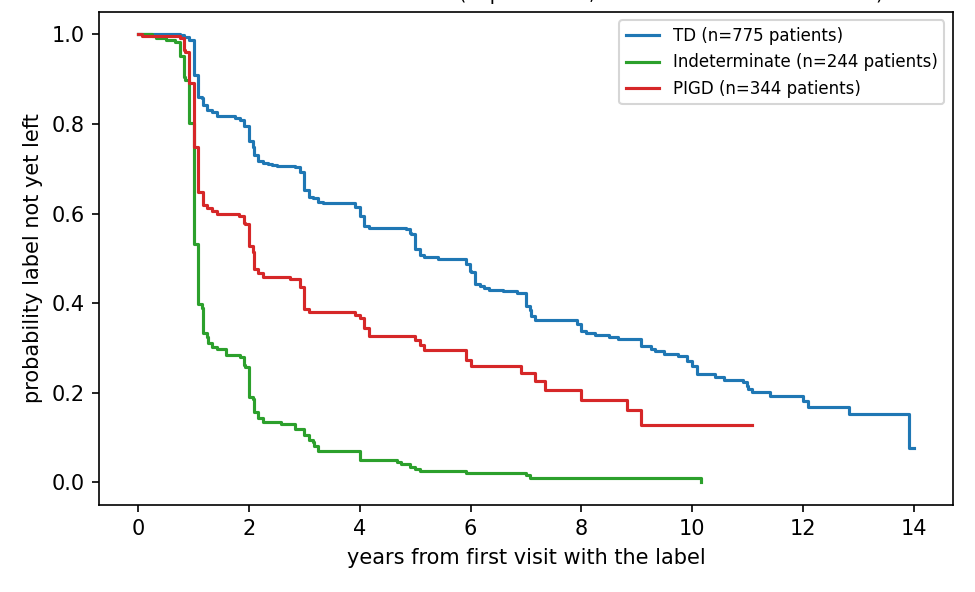
\includegraphics[width=0.80\textwidth]{s02_exit_ind.png}
\caption{Kaplan--Meier time to the first different recorded label, by the label
held at entry, censored at the last labelled visit. The Indeterminate label is
left far faster than either extreme label.}
\label{sfig:exit}
\end{figure}

Figure~\ref{sfig:reversion} gives the reversion rates by type of change that
underlie panel (a) of Table~\ref{tab:dynamics}.

\begin{figure}[htbp]
\centering
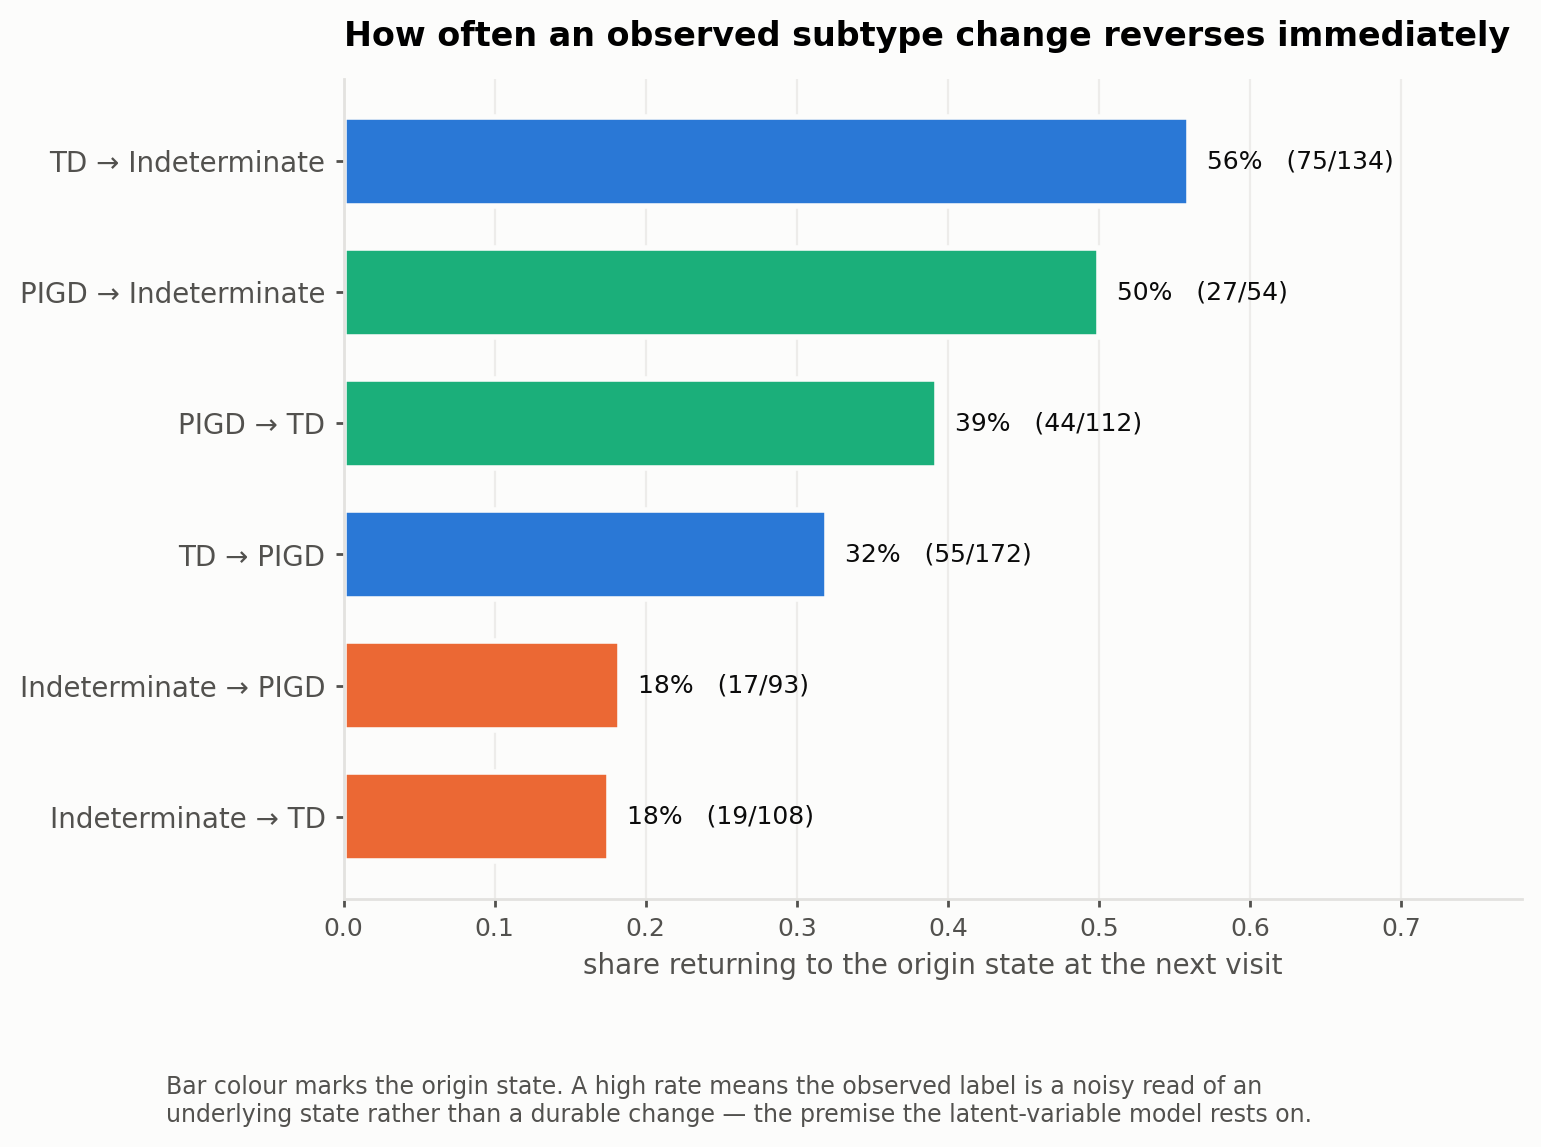
\includegraphics[width=0.80\textwidth]{s01_reversion.png}
\caption{Proportion of observed changes that return to the origin label at the
following visit, by type of change, with patient-clustered bootstrap 95\%
intervals. Changes into the Indeterminate band revert at about half, changes
crossing the full width of the scale at about a third.}
\label{sfig:reversion}
\end{figure}

\paragraph{Limitation.} The clustering statistic has low power at 441
Indeterminate visits, so the inconclusive verdict reflects the design as much as
the data.

% --------------------------------------------------------------------
\section{Localising the generative misfit}
\label{sup:ppc}
% --------------------------------------------------------------------

Section~\ref{sec:ppc} reports that a hierarchical growth model of the ratio with
Student-t slopes and residuals fails a pre-registered posterior-predictive check.
Diagnostics localise the misfit without attaching a verdict.

\paragraph{The Indeterminate excess is a lattice effect.} The excess of 183
Indeterminate visits over the generator's expectation is concentrated at PIGD
item sums 2 (50\% of the excess), 3 (24\%) and 4--5 (22\%); at sum 1 the observed
and expected counts agree (70 against 71.8). Within each stratum the
Indeterminate cells of the lattice hold about as many visits as their
neighbouring cells, so the Indeterminate visits are ordinary lattice points
rather than a local concentration. A band of nominal width 0.25 captures 1.82
times its width in lattice points at PIGD sums 1 and 2; correcting for that
inflation gives an expected share of about 0.068, two thirds of the way from the
observed 0.103 to the generator's 0.051. The whole gap in the ratio distribution
opens inside $(0.90, 1.15]$ and closes again above 2.

\paragraph{The reversion deficit is direction-specific.}
Figure~\ref{sfig:direction} gives the outcome of direct TD--PIGD changes by
direction. TD-to-PIGD changes revert at 0.253 (0.187--0.325) against a generator
expectation of 0.469 --- 37 observed reversions against 83 expected --- whereas
PIGD-to-TD changes revert at 0.398 against an expectation of 0.396. There are
also fewer direct changes overall than the generator implies (244 against 315
with an observed outcome). A symmetric-noise model of a continuous quantity
cannot produce an asymmetry of this kind.

\begin{figure}[htbp]
\centering
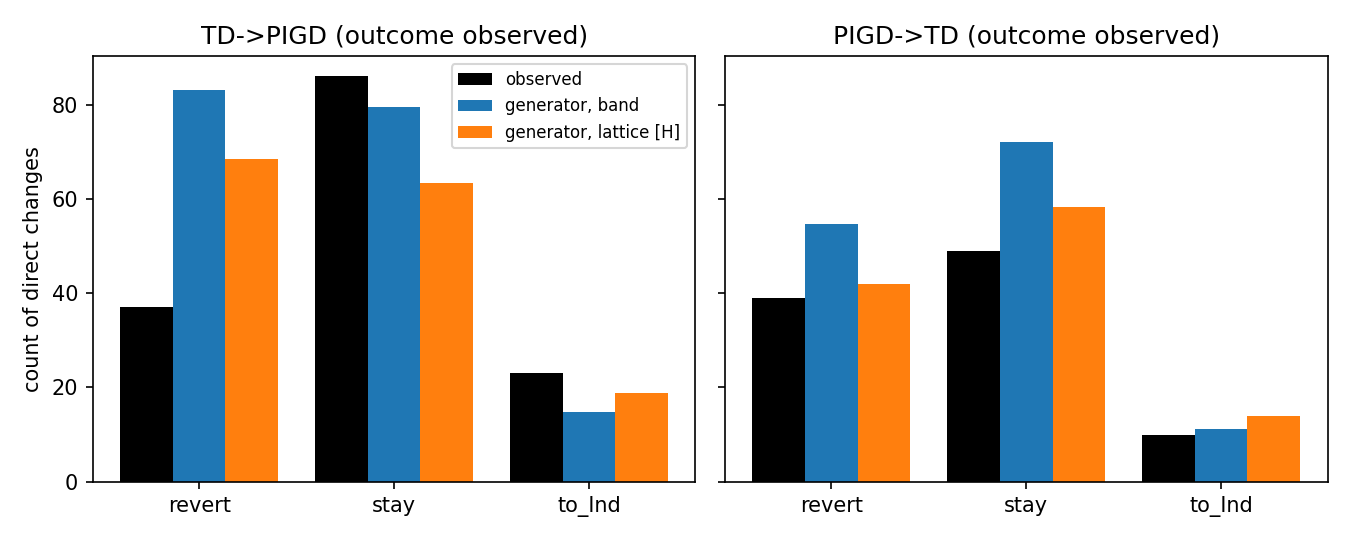
\includegraphics[width=\textwidth]{s03_direction.png}
\caption{Outcome of direct TD--PIGD changes by direction: observed counts against
the expectation under the fitted continuous-ratio generator, treating the band as
a continuous interval and as its lattice catchment. The deficit of observed
reversions is confined to the TD-to-PIGD direction.}
\label{sfig:direction}
\end{figure}

\paragraph{Two caveats.} The diagnostic reference is the covariate-blind generator
rather than the patient-conditional replicate distribution the check itself used,
because the replicate labels were not saved; the re-execution that would have
saved them is described in \ref{sup:notrun}. A valid Student-t residual
diagnostic was not possible from the saved outputs because the fold posteriors of
the random effects were not retained. The misfit is present, and larger, among
the 585 patients with no excluded PIGD-zero visit, which weakens the exclusion of
Section~\ref{sec:undefined} as its driver.

% --------------------------------------------------------------------
\section{Fitted parameters, the emission floor and model stability}
\label{sup:hmm}
% --------------------------------------------------------------------

\subsection{Fitted parameters and the first split}
Table~\ref{stab:hmm} gives the fitted misclassification matrix, the generators
and mean sojourn times of the observed-label and latent chains, and the held-out
performance on the single 70/30 patient split that preceded the
leave-one-patient-out protocol.

Three points follow. The latent generator differs sharply from the observed-label
generator: the latent TD state leaves for PIGD directly at 0.006 per year against
0.058 for the recorded label, and implied mean sojourns are 10.1, 2.1 and 16.5
years in the latent states against 3.4, 0.4 and 2.3 years in the recorded label.
Horizon probabilities computed from the latent generator are latent-to-latent and
\textbf{must not} be read as probabilities of the recorded label: the latent
five-year probability of PIGD given TD is 0.191, whereas the recorded-label chain
gives 0.296.

On the first split the latent-state model reached $-0.638$ log-likelihood per
pair against $-0.665$ for the discrete chain and $-0.675$ for the continuous
chain, and across ten further random splits it beat the discrete chain on every
one, by $+0.028$ per pair on average (SD 0.009). The continuous-time chain
\emph{without} a latent layer loses to the discrete chain at every interval
stratum, because the discrete chain's ``next visit'' absorbs the attendance
schedule that the continuous chain has to model with six rates.

\begin{table}[htbp]
\centering
\caption{Fitted parameters of the three-state hidden Markov model and held-out
performance on the first 70/30 patient split.}
\label{stab:hmm}
\small
\begin{tabular}{@{}lrrr@{}}
\toprule
\multicolumn{4}{@{}l}{\textit{(a) Fitted misclassification matrix $E$ (rows: latent state)}}\\
Latent state & $\Pr(Y{=}\TD)$ & $\Pr(Y{=}\Ind)$ & $\Pr(Y{=}\PIGD)$ \\
\midrule
TD            & 0.9412 & 0.0383 & 0.0205 \\
Indeterminate & 0.2500 & \textbf{0.5000} & 0.2500 \\
PIGD          & 0.1056 & 0.0520 & 0.8424 \\
\midrule
\multicolumn{4}{@{}l}{\textit{(b) Off-diagonal rates (per year) and mean sojourn times (years)}}\\
Quantity & \multicolumn{1}{c}{Observed-label chain} & \multicolumn{2}{c}{Latent chain} \\
\midrule
TD $\to$ Indeterminate            & 0.2348 & \multicolumn{2}{r}{0.0937} \\
TD $\to$ PIGD                     & 0.0583 & \multicolumn{2}{r}{0.0057} \\
Indeterminate $\to$ TD            & 1.2212 & \multicolumn{2}{r}{0.1156} \\
Indeterminate $\to$ PIGD          & 1.0689 & \multicolumn{2}{r}{0.3557} \\
PIGD $\to$ TD                     & 0.0880 & \multicolumn{2}{r}{0.0000} \\
PIGD $\to$ Indeterminate          & 0.3499 & \multicolumn{2}{r}{0.0605} \\
\addlinespace[2pt]
Mean sojourn, TD                  & 3.41 & \multicolumn{2}{r}{10.06} \\
Mean sojourn, Indeterminate       & 0.44 & \multicolumn{2}{r}{2.12} \\
Mean sojourn, PIGD                & 2.28 & \multicolumn{2}{r}{16.52} \\
\midrule
\multicolumn{4}{@{}l}{\textit{(c) Held-out performance on the 70/30 split (1,002 pairs)}}\\
Model & Log-lik.\ / pair & Accuracy & Brier \\
\midrule
Hidden Markov model               & $-0.6384$ & 0.7695 & 0.3458 \\
Markov chain, discrete-time       & $-0.6653$ & 0.7675 & 0.3625 \\
Markov chain, continuous-time     & $-0.6752$ & 0.7655 & 0.3670 \\
Marginal null                     & $-0.8633$ & 0.6248 & 0.5185 \\
\multicolumn{4}{@{}l}{Across ten further splits: HMM $-$ discrete chain $= +0.0284$ (SD 0.0094), positive in 10 of 10.}\\
\bottomrule
\end{tabular}

\end{table}

\begin{figure}[htbp]
\centering
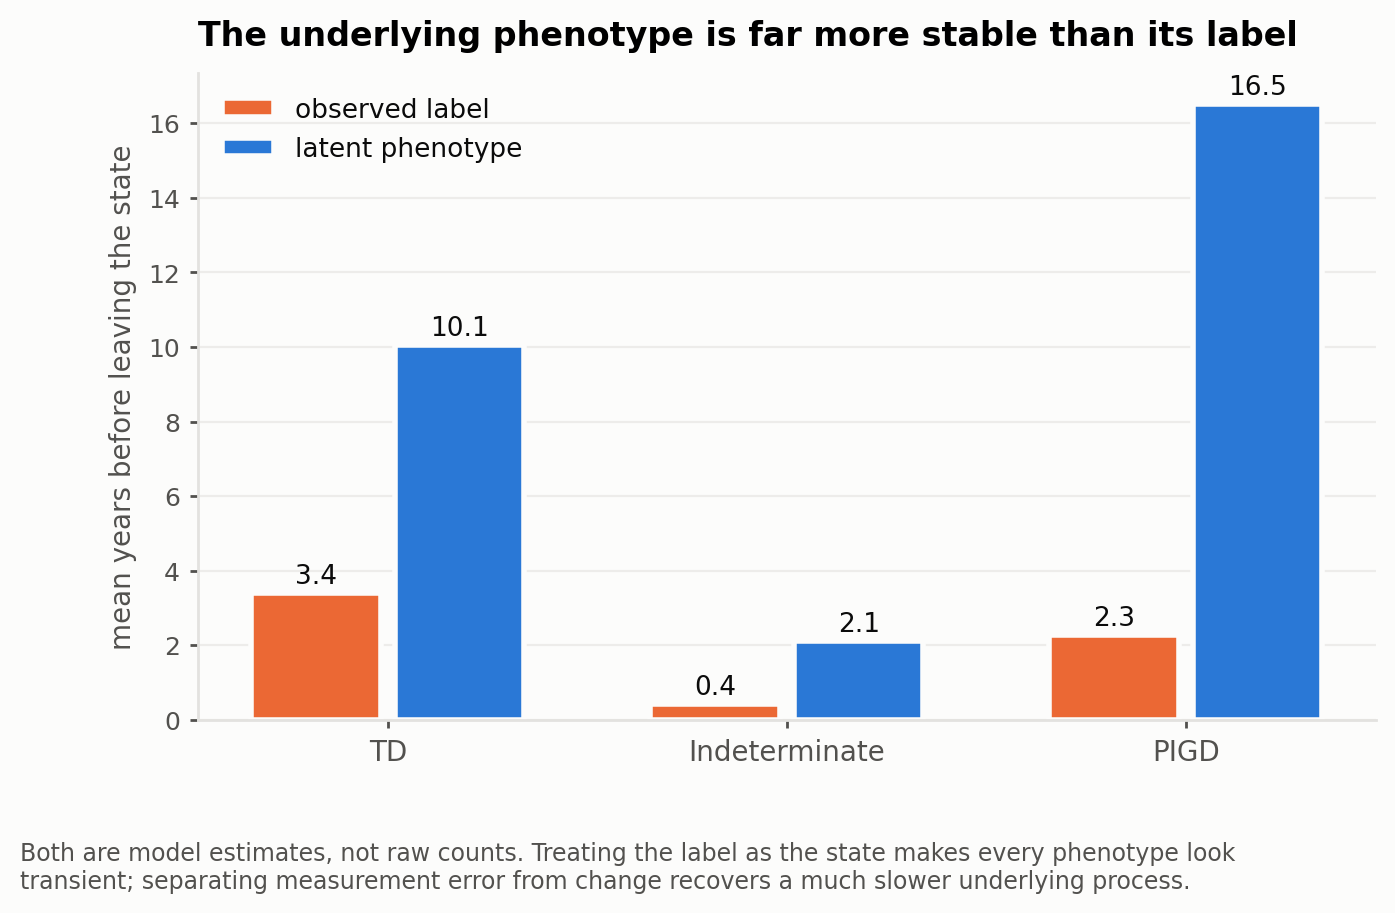
\includegraphics[width=0.80\textwidth]{s04_sojourn.png}
\caption{Mean sojourn times implied by the chain in the recorded label and by the
latent chain of the hidden Markov model. The latent states are far more
persistent than the labels that read them, which is the model's account of the
label's instability.}
\label{sfig:sojourn}
\end{figure}

\subsection{Is the optimum unique, and do more states help?}
Table~\ref{stab:stability} reports 40 random restarts per configuration on the
full cohort and the held-out performance of each configuration.

The three-state floor-constrained fit has a \emph{unique} optimum: all 40 starts
reach the same log-likelihood to within 0.01, with generator entries agreeing to
0.0014 and emission entries to 0.0003. Without the floor the three-state fit sits
on a ridge --- 38 of 40 starts are within 0.01 of the best, yet their emission
entries differ by up to 0.93 --- and the five-state fit is multimodal, with one
of 40 starts within 0.01 of the best and 36 distinct optima at that resolution.

On held-out prediction every configuration is equivalent: accuracies between
0.752 and 0.755 and log-likelihoods between $-0.669$ and $-0.675$. A nested
selection procedure that chose the unconstrained three-state model in eight outer
folds and the five-state model in two reaches 0.755, the same as the audited
model. \textbf{The floor therefore buys identifiability, not accuracy.}

A prior-corrected decision rule that divides each predicted probability by its
class prevalence recovers Indeterminate recall of 0.25 to 0.32 at the cost of
accuracy, which falls to 0.68--0.71. The predicted probabilities themselves do
not change, which locates the failure to predict the minority class in the
interaction between the argmax rule and a rare class, not in the fitted model.

\begin{table}[htbp]
\centering
\caption{Stability of the fitted optimum across random restarts, and held-out
performance of alternative configurations under the argmax rule and under a
prior-corrected rule.}
\label{stab:stability}
\small
\begin{tabular}{@{}lrrrrrr@{}}
\toprule
\multicolumn{7}{@{}l}{\textit{(a) Full-cohort fits from 40 random starts per configuration}}\\
Configuration & Par. & Best log-lik. & Worst log-lik. & Within 0.01 & Optima & Max $|\Delta E|$ \\
\midrule
3 states, floor 0.5 & 14 & $-2969.06$ & $-2969.06$ & 1.000 & 1  & 0.0003 \\
3 states, floor 0.6 & 14 & $-2974.77$ & $-3657.69$ & 0.975 & 2  & 0.0002 \\
3 states, floor 0.7 & 14 & $-2979.10$ & $-3657.69$ & 0.975 & 2  & 0.0000 \\
3 states, free      & 14 & $-2955.32$ & $-2955.45$ & 0.950 & 2  & \textbf{0.9280} \\
4 states, free      & 23 & $-2947.37$ & $-2954.83$ & 0.600 & 15 & 0.0050 \\
5 states, free      & 34 & $-2938.82$ & $-2953.92$ & \textbf{0.025} & \textbf{36} & 0.0000 \\
\midrule
\multicolumn{7}{@{}l}{\textit{(b) Held-out performance of each configuration (argmax rule)}}\\
Configuration & \multicolumn{2}{l}{Accuracy} & \multicolumn{2}{l}{95\% CI} & Bal.\ acc. & Rec.\ Ind. \\
\midrule
3 states, floor 0.5 & \multicolumn{2}{l}{0.7542} & \multicolumn{2}{l}{(0.7351, 0.7734)} & 0.5259 & 0.000 \\
3 states, free      & \multicolumn{2}{l}{0.7539} & \multicolumn{2}{l}{(0.7341, 0.7733)} & 0.5222 & 0.000 \\
4 states, free      & \multicolumn{2}{l}{0.7525} & \multicolumn{2}{l}{(0.7327, 0.7715)} & 0.5222 & 0.000 \\
5 states, free      & \multicolumn{2}{l}{0.7542} & \multicolumn{2}{l}{(0.7348, 0.7732)} & 0.5256 & 0.000 \\
\midrule
\multicolumn{7}{@{}l}{\textit{(c) A prior-corrected decision rule recovers the minority class at a cost}}\\
3 states, floor 0.5 & \multicolumn{2}{l}{0.7123} & \multicolumn{2}{l}{(0.6912, 0.7342)} & 0.5706 & \textbf{0.253} \\
3 states, free      & \multicolumn{2}{l}{0.6897} & \multicolumn{2}{l}{(0.6662, 0.7139)} & 0.5709 & 0.307 \\
5 states, free      & \multicolumn{2}{l}{0.6807} & \multicolumn{2}{l}{(0.6558, 0.7065)} & 0.5702 & 0.319 \\
\bottomrule
\end{tabular}

\end{table}

\subsection{The five-state leave-one-patient-out run}
The five-state specification re-scored in the harmonised comparison reached
0.7513, below the three-state model. Its fits converged in only 404 of 934 folds,
so 59.2\% of its predictions come from non-converged fits. It is reported as a
negative result about model capacity and is not used to support any other claim.

\begin{figure}[htbp]
\centering
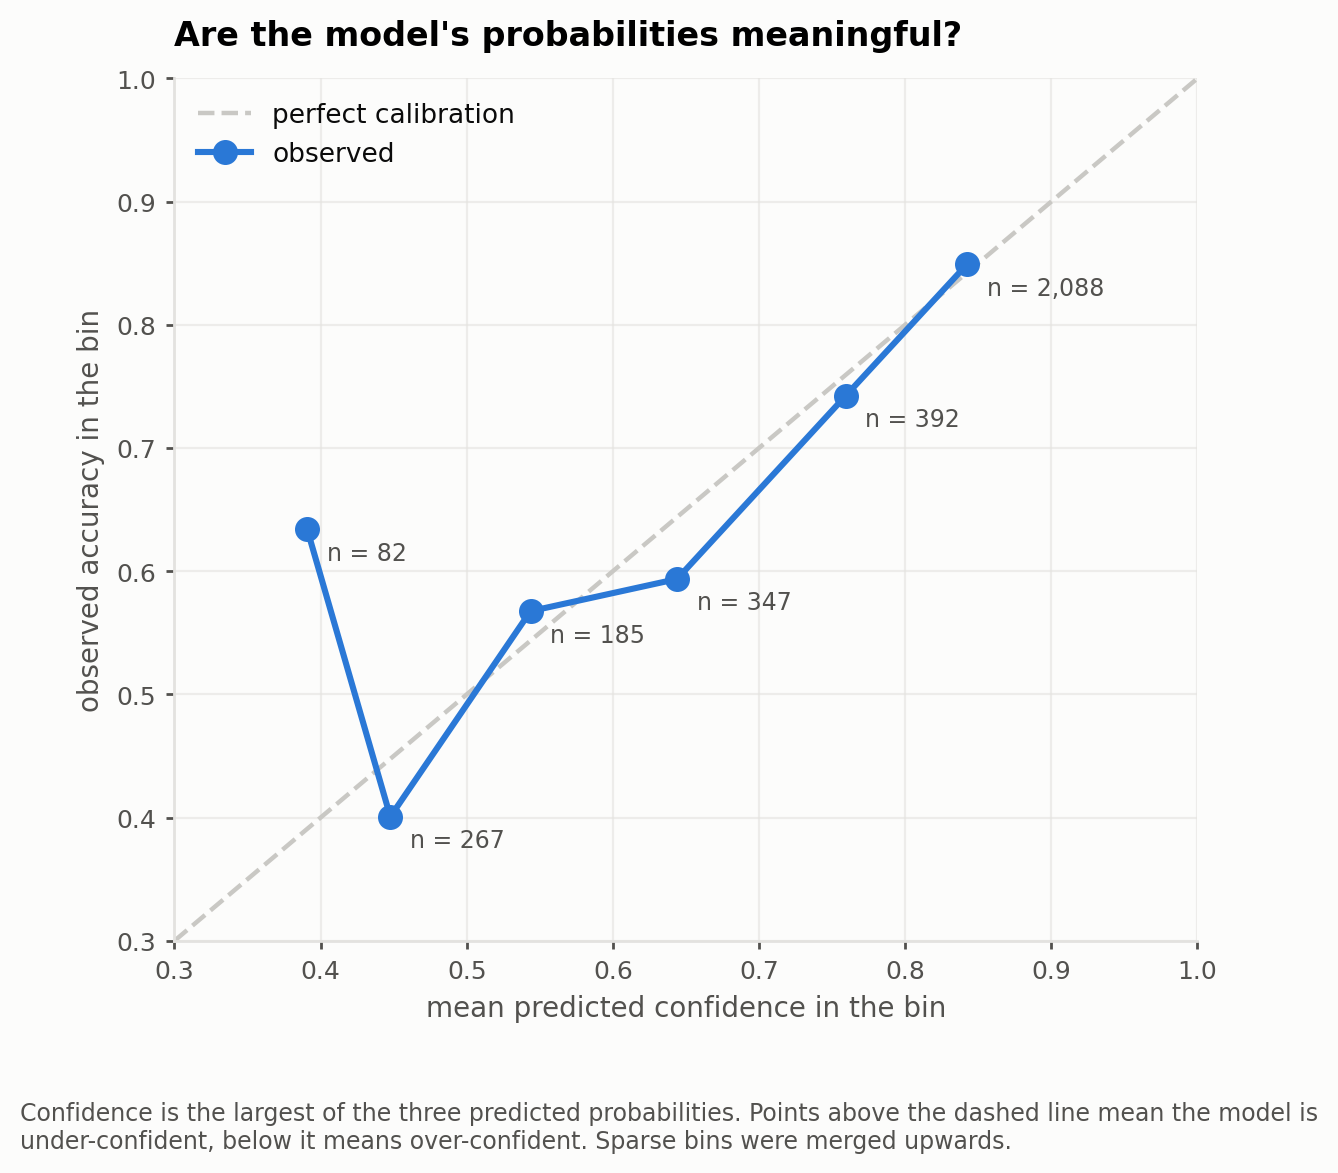
\includegraphics[width=0.74\textwidth]{s05_calibration.png}
\caption{Calibration of the hidden Markov model's maximum predicted probability
under leave-one-patient-out. The reliability curve is close to the diagonal at
the confidence levels the model actually uses.}
\label{sfig:calib}
\end{figure}

% --------------------------------------------------------------------
\section{Prediction with no history}
\label{sup:firstvisit}
% --------------------------------------------------------------------

What can be predicted at a patient's first visit, before any longitudinal
information exists, bounds what the longitudinal models add.

Averaged over ten random 70/30 splits (Table~\ref{stab:firstvisit}), a lookup of
the current label and the prediction horizon gives $-0.781$ log-likelihood per
prediction; adding the baseline ratio gives $-0.773$, adding ten baseline
clinical measures $-0.763$, and both $-0.755$, against $-0.787$ for the hidden
Markov model given no history --- a gain of 0.032 per prediction for the full
first-visit model.

The MDS-UPDRS Part II total is the only covariate whose removal costs more than
0.01 per prediction. DaTscan putamen binding, age and Hoehn \& Yahr stage cost
0.005, 0.004 and 0.002, and the cognitive, olfactory, autonomic and sleep
measures cost nothing or less than nothing. \textbf{None of the
diffuse-synucleinopathy markers predicts the motor label.} Accuracy falls with
horizon from 0.776 within 1.5 years to 0.616 beyond 6.5 years.

\begin{table}[htbp]
\centering
\caption{First-visit prediction with no longitudinal history.}
\label{stab:firstvisit}
\small
\begin{tabular}{@{}lrr@{}}
\toprule
\multicolumn{3}{@{}l}{\textit{(a) Nested first-visit models: held-out log-likelihood per prediction (mean of 10 splits)}}\\
Model & Mean & SD across splits \\
\midrule
Hidden Markov model, no history       & $-0.7869$ & 0.0246 \\
Current subtype $+$ horizon           & $-0.7813$ & 0.0280 \\
\quad $+$ baseline ratio              & $-0.7735$ & 0.0311 \\
\quad $+$ ten baseline covariates     & $-0.7625$ & 0.0378 \\
\quad $+$ ratio $+$ covariates        & $\mathbf{-0.7550}$ & 0.0416 \\
\midrule
\multicolumn{3}{@{}l}{\textit{(b) Cost of dropping each covariate (log-likelihood per prediction)}}\\
Covariate & \multicolumn{2}{r}{Cost of dropping} \\
\midrule
MDS-UPDRS Part II total               & \multicolumn{2}{r}{0.0153} \\
DaTscan putamen binding, bilateral    & \multicolumn{2}{r}{0.0050} \\
Age                                   & \multicolumn{2}{r}{0.0042} \\
Hoehn \& Yahr stage                   & \multicolumn{2}{r}{0.0021} \\
Sex                                   & \multicolumn{2}{r}{0.0002} \\
MoCA, UPSIT, disease duration, SCOPA-AUT, RBDSQ & \multicolumn{2}{r}{$\leq 0$} \\
\midrule
\multicolumn{3}{@{}l}{\textit{(c) Performance by prediction horizon (main split)}}\\
Horizon & $n$ & Accuracy \\
\midrule
$<1.5$ y        & 241 & 0.7759 \\
1.5--3.5 y      & 358 & 0.7570 \\
3.5--6.5 y      & 218 & 0.6789 \\
$>6.5$ y        & 185 & 0.6162 \\
\bottomrule
\end{tabular}

\end{table}

\paragraph{Limitations.} Covariates are mean-imputed within the training split,
and this model was not run under leave-one-patient-out, so its figures are not
directly comparable with the main text's.

% --------------------------------------------------------------------
\section{Student-t variants of the growth model}
\label{sup:studentt}
% --------------------------------------------------------------------

Four variants of the growth model~\eqref{eq:hb} were compared over seven patient
splits, crossing Gaussian or Student-t patient slopes with Gaussian or Student-t
residuals (Table~\ref{stab:studentt}).

\paragraph{Residual tails: supported.} Replacing Gaussian residuals with Student-t
residuals improves held-out prediction unambiguously --- $+0.112$ log predictive
density per visit ($+0.061$ to $+0.168$) with Gaussian slopes, and $+0.106$
($+0.058$ to $+0.158$) with Student-t slopes, positive in all seven splits --- and
improves the class-label metric by about $+0.038$. The fitted residual degrees of
freedom are about 2.1.

\paragraph{Slope tails: not supported.} The original sampler for the slope degrees
of freedom did not converge ($\hat{R} = 1.018$, effective sample size 248) and the
question was declared inconclusive. A pre-registered reassessment with a collapsed
slice sampler converged ($\hat{R} = 1.004$, effective sample size 937) and found a
full-cohort posterior median of 2.09 (1.48--4.11), but met the per-split decision
criterion in only one of seven splits against a threshold of five. The procedure
was calibrated: zero false flags in 180 null cohorts across three scenarios, and
55 of 60 detections in the positive control. The verdict is \textbf{not
supported}.

\paragraph{Why this matters.} The heavy residual tails are the same phenomenon the
lag-1 residual analysis and the posterior-predictive check see from different
directions: occasional large excursions of the ratio that do not persist to the
next visit. They are a property of the measurement, not of patient-level
heterogeneity in progression rate --- which is exactly what the negative result on
slope tails says.

\begin{table}[htbp]
\centering
\caption{Student-t variants of the growth model over seven patient splits. GG,
GT, TG and TT denote Gaussian or Student-t slopes and residuals respectively.}
\label{stab:studentt}
\small
\begin{tabular}{@{}lllr@{}}
\toprule
Question & Quantity & Estimate (95\% interval) & Splits \\
\midrule
\multicolumn{4}{@{}l}{\textit{(a) Are the residuals heavy-tailed? (Q1)}}\\
 & GT $-$ GG, log predictive density per visit & $+0.1115$ ($+0.0606$, $+0.1676$) & 7/7 \\
 & GT $-$ GG, class-label metric              & $+0.0382$ ($+0.0205$, $+0.0549$) & 7/7 \\
 & TT $-$ TG, log predictive density per visit & $+0.1060$ ($+0.0577$, $+0.1575$) & 7/7 \\
 & TT $-$ TG, class-label metric              & $+0.0379$ ($+0.0212$, $+0.0546$) & 7/7 \\
 & \multicolumn{3}{l}{\textbf{Verdict: supported.} Residual degrees of freedom $\approx 2.1$.} \\
\addlinespace[3pt]
\multicolumn{4}{@{}l}{\textit{(b) Are the patient slopes heavy-tailed? (Q2)}}\\
 & Original run: $\hat{R}$ / effective sample size & 1.018 / 248 & inconclusive \\
 & Reassessment: $\hat{R}$ / effective sample size & 1.0044 / 937 & converged \\
 & Full-cohort posterior median $\nu_{\mathrm{slope}}$ & 2.09 (1.48, 4.11) & --- \\
 & Per-split criterion met ($\nu$ upper bound $<10$) & 1 of 7 & threshold 5/7 \\
 & Null calibration, scenarios C1--C3 & 0 flags in 180 cohorts & --- \\
 & Positive control, scenario P & 55 of 60 detected & --- \\
 & \multicolumn{3}{l}{\textbf{Verdict: not supported.} No evidence of extreme slope tails.} \\
\addlinespace[3pt]
\multicolumn{4}{@{}l}{\textit{(c) Predictive value of each variant against the Gaussian model (Q3)}}\\
 & TG, class-label metric & $+0.0034$ ($+0.0007$, $+0.0063$) & 6/7 \\
 & GT, class-label metric & $+0.0382$ ($+0.0205$, $+0.0549$) & 7/7 \\
 & TT, class-label metric & $+0.0412$ ($+0.0229$, $+0.0586$) & 7/7 \\
\bottomrule
\end{tabular}

\end{table}

% --------------------------------------------------------------------
\section{The full subscore comparison}
\label{sup:subscore}
% --------------------------------------------------------------------

Table~\ref{stab:subscore} gives the fifteen-arm held-out comparison of subscore
models on identical points, the pre-specified paired contrasts, the derived-label
contrasts against the hidden Markov model, and the parameters of the joint
bivariate mixed model.

\paragraph{The cross-output block is worth nothing.} The full coregionalisation
block is indistinguishable from its diagonal counterpart on every metric and both
outcomes: the largest effect is a change of $-0.0002$ in tremor CRPS. The reason
is that the two subscores are nearly uncorrelated, with a random-intercept
correlation of $-0.015$ and a residual correlation of $+0.019$. All 3,736
multi-output fits converged.

\paragraph{Temporal flexibility helps the proper scores, not the absolute error.}
Kernels carrying both a linear term and a flexible component ($K_2$, $K_3$) beat
the simpler ones on CRPS and log score for both outcomes --- joint log score
$+0.073$ ($+0.051$ to $+0.096$) for $K_2$ against $K_0$ --- while MAE moves by
thousandths. Every Gaussian process beats persistence on CRPS and log score, and
loses to it on PIGD absolute error.

\paragraph{The interpretable parametric comparator loses.} The joint bivariate
mixed model estimates population slopes of $+0.023$ per year for tremor and
$+0.066$ for PIGD, with intraclass correlations of 0.61 and 0.45. Its held-out
MAE is worse than persistence on both outcomes ($+0.012$ and $+0.035$), and its
derived label is worse than the hidden Markov model on log loss ($+0.018$,
$+0.004$ to $+0.032$).

\paragraph{The derived label under two rules.} Classifying the point prediction
gives 0.730 accuracy and recovers Indeterminate at recall 0.17; taking the argmax
of the Monte Carlo probability vector gives 0.757 and recovers it at 0.000. The
two rules differ by more than the entire spread between fitted models, which is
why the main text harmonises on one of them (Section~\ref{sec:harmonisation}).

\begin{table}[htbp]
\centering
\caption{The full subscore comparison on identical leave-one-patient-out points.}
\label{stab:subscore}
\footnotesize
\begin{tabular}{@{}llrrrr@{}}
\toprule
Outcome & Model & MAE & CRPS & Log score & Cov.\ 95\% \\
\midrule
\multicolumn{6}{@{}l}{\textit{(a) Fifteen-arm held-out comparison (934 patients, 3,361 points)}}\\
tremor & GP, $K_0$              & 0.2385 & 0.1716 & $-0.2482$ & 0.939 \\
tremor & GP, $K_1$              & 0.2395 & 0.1708 & $-0.2392$ & 0.936 \\
tremor & GP, $K_2$              & 0.2358 & 0.1689 & $-0.2264$ & 0.937 \\
tremor & GP, $K_3$              & 0.2359 & 0.1690 & $-0.2262$ & 0.937 \\
tremor & GP, joint $K_1$ full   & 0.2391 & 0.1706 & $-0.2378$ & 0.936 \\
tremor & Mixed model (RI)       & 0.2546 & 0.1817 & $-0.3151$ & 0.935 \\
tremor & Patient mean           & 0.2498 & 0.1830 & $-0.3158$ & 0.926 \\
tremor & Persistence            & 0.2426 & 0.1797 & $-0.3024$ & 0.953 \\
\addlinespace[2pt]
pigd   & GP, $K_0$              & 0.2156 & 0.1634 & $-0.2848$ & 0.944 \\
pigd   & GP, $K_1$              & 0.2175 & 0.1618 & $-0.2648$ & 0.933 \\
pigd   & GP, $K_2$              & 0.2132 & 0.1601 & $-0.2339$ & 0.939 \\
pigd   & GP, $K_3$              & 0.2129 & 0.1599 & $-0.2334$ & 0.939 \\
pigd   & GP, joint $K_1$ full   & 0.2173 & 0.1617 & $-0.2644$ & 0.933 \\
pigd   & Mixed model (RI)       & 0.2391 & 0.1809 & $-0.4225$ & 0.940 \\
pigd   & Patient mean           & 0.2400 & 0.1985 & $-0.5281$ & 0.932 \\
pigd   & Persistence            & \textbf{0.2040} & 0.1724 & $-0.3486$ & 0.951 \\
\midrule
\multicolumn{6}{@{}l}{\textit{(b) Pre-specified paired contrasts}}\\
\multicolumn{2}{@{}l}{Cross-output block vs its diagonal ($K_1$, tremor, CRPS)}
   & \multicolumn{4}{l}{$-0.0002$ ($-0.0003$, $+0.0000$) \quad neither} \\
\multicolumn{2}{@{}l}{Temporal flexibility, $K_2 - K_0$ (joint log score)}
   & \multicolumn{4}{l}{$+0.0726$ ($+0.0511$, $+0.0957$) \quad \textbf{model}} \\
\multicolumn{2}{@{}l}{$K_1 -$ persistence (joint log score)}
   & \multicolumn{4}{l}{$+0.1437$ ($+0.1020$, $+0.1860$) \quad \textbf{model}} \\
\midrule
\multicolumn{6}{@{}l}{\textit{(c) Derived three-class label vs the hidden Markov model on the same 3,361 points}}\\
\multicolumn{2}{@{}l}{GP $K_1$, accuracy (argmax)} & \multicolumn{4}{l}{$+0.0024$ ($-0.0045$, $+0.0092$)} \\
\multicolumn{2}{@{}l}{GP joint $K_1$, accuracy (argmax)} & \multicolumn{4}{l}{$+0.0045$ ($-0.0026$, $+0.0117$)} \\
\multicolumn{2}{@{}l}{GP $K_1$, log loss} & \multicolumn{4}{l}{$-0.0196$ ($-0.0317$, $-0.0073$) \quad \textbf{favours the GP}} \\
\multicolumn{2}{@{}l}{Mixed model, log loss} & \multicolumn{4}{l}{$+0.0177$ ($+0.0035$, $+0.0324$) \quad \textbf{favours the HMM}} \\
\midrule
\multicolumn{6}{@{}l}{\textit{(d) Joint bivariate mixed model: fixed effects (934 patients, 8,590 observations)}}\\
\multicolumn{2}{@{}l}{Tremor intercept / slope per year}
   & \multicolumn{4}{l}{0.5841 (0.5594, 0.6089) \,/\, $+0.0233$ ($+0.0202$, $+0.0265$)} \\
\multicolumn{2}{@{}l}{PIGD intercept / slope per year}
   & \multicolumn{4}{l}{0.2301 (0.2085, 0.2517) \,/\, $+0.0655$ ($+0.0621$, $+0.0689$)} \\
\multicolumn{2}{@{}l}{Random-intercept / residual correlation}
   & \multicolumn{4}{l}{$-0.0153$ \,/\, $+0.0186$} \\
\multicolumn{2}{@{}l}{Intraclass correlation, tremor / PIGD}
   & \multicolumn{4}{l}{0.6067 \,/\, 0.4527} \\
\bottomrule
\end{tabular}

\end{table}

\paragraph{Limitations.} Raw-scale Gaussian likelihoods on bounded, zero-inflated
scores; the derived label uses Monte Carlo through a ratio of two Gaussians
clipped at zero; the subscore models train on 934 patients and the ratio model on
821, so their absolute errors are not comparable with each other.

% --------------------------------------------------------------------
\section{Time-varying rates and their identifiability}
\label{sup:temporal}
% --------------------------------------------------------------------

Table~\ref{stab:temporal} reports the period-specific slopes of the two subscores
under a linear-spline mixed model, the within-patient change in rate, a dedicated
identifiability audit, and an attrition model.

\paragraph{The population pattern is clear.} The PIGD slope rises across follow-up
(0.045, 0.057 and 0.080 per year in years 0--2, 2--5 and beyond 5) and the tremor
slope falls (0.033, 0.033 and 0.013). The contrasts between the last and the first
period are $+0.035$ for PIGD and $-0.020$ for tremor, and within the 226 patients
observed in both periods the PIGD rate rises by $+0.073$ ($+0.043$ to $+0.101$)
and the tremor rate falls by $-0.040$ ($-0.073$ to $-0.008$). So the pattern is
within patients as well as between them (Figure~\ref{sfig:slopes}).

\paragraph{But it is not identifiable, not honest, and not predictive.} A
supremum likelihood-ratio test confirms a departure from linearity (39.1 against
a bootstrap 95th percentile of 7.7 under a random-intercept null and 20.4 under a
random-slope null, $P = 0.005$ under both), but the best single knot sits at 4.75
years with a bootstrap range of 2.5 to 10 years, and a quadratic mean is preferred
by AIC over a linear one by 37.8 units. The Wald intervals on the late-period
slopes are too narrow by factors of 1.7 (tremor) and 2.2 (PIGD) against a patient
bootstrap. Attrition is informative: the log-odds of loss to follow-up after a
visit rise by $+0.52$ ($+0.36$ to $+0.71$) per point of PIGD score. On a
disease-duration time axis the slope changes at five years no longer exclude zero,
and the treated share rises from 0.10 at baseline to 0.95 by year five, so the
acceleration is confounded with duration and treatment.

Held out, the spline improves PIGD absolute error over the constant-rate model by
$-0.0034$ ($-0.0044$ to $-0.0023$) and tremor not at all, and both lose to
persistence; the derived label is 0.709 under either. \textbf{This is a population
description, not a predictive feature}, and it is why no time-varying structure
enters the prediction models of the main text.

\begin{table}[htbp]
\centering
\caption{Time-varying rates of the two subscores, and the audit of their
identifiability and interval coverage.}
\label{stab:temporal}
\small
\begin{tabular}{@{}llrll@{}}
\toprule
Outcome & Period & Slope / y & Wald 95\% CI & Patient-bootstrap 95\% CI \\
\midrule
\multicolumn{5}{@{}l}{\textit{(a) Period-specific population slopes (knots at 2 and 5 years)}}\\
tremor & 0--2 y  & 0.0327 & (0.0196, 0.0458) & (0.0201, 0.0450) \\
tremor & 2--5 y  & 0.0325 & (0.0212, 0.0439) & (0.0189, 0.0458) \\
tremor & $>$5 y  & 0.0126 & (0.0056, 0.0197) & (0.0001, 0.0238) \\
pigd   & 0--2 y  & 0.0450 & (0.0309, 0.0592) & (0.0348, 0.0564) \\
pigd   & 2--5 y  & 0.0574 & (0.0453, 0.0695) & (0.0429, 0.0733) \\
pigd   & $>$5 y  & 0.0800 & (0.0724, 0.0875) & (0.0640, 0.0971) \\
\addlinespace[2pt]
\multicolumn{5}{@{}l}{SE ratio, bootstrap / Wald, late period: tremor 1.72, PIGD 2.23.}\\
\midrule
\multicolumn{5}{@{}l}{\textit{(b) Within-patient change in rate (patients observed in both periods)}}\\
pigd   & 0--2 $\to$ $>$5 y & $+0.0727$ & \multicolumn{2}{l}{($+0.0425$, $+0.1014$), $n = 226$} \\
tremor & 0--2 $\to$ $>$5 y & $-0.0396$ & \multicolumn{2}{l}{($-0.0731$, $-0.0079$), $n = 226$} \\
\midrule
\multicolumn{5}{@{}l}{\textit{(c) Is the change in rate identifiable?}}\\
\multicolumn{2}{@{}l}{Supremum likelihood ratio} & 39.13 & \multicolumn{2}{l}{$P = 0.005$ under both null models} \\
\multicolumn{2}{@{}l}{Null 95th percentile} & 7.68 / 20.39 & \multicolumn{2}{l}{random-intercept / random-slope null} \\
\multicolumn{2}{@{}l}{Best single knot} & 4.75 y & \multicolumn{2}{l}{bootstrap 2.5--97.5 pct: 2.5 to 10 y} \\
\multicolumn{2}{@{}l}{Held-out gain over a linear trend} & \multicolumn{3}{l}{PIGD MAE $-0.0034$; tremor none; both lose to persistence} \\
\midrule
\multicolumn{5}{@{}l}{\textit{(d) Attrition after a visit (logistic, bootstrap intervals)}}\\
\multicolumn{2}{@{}l}{Years from baseline} & $+0.1386$ & \multicolumn{2}{l}{($+0.1221$, $+0.1576$)} \\
\multicolumn{2}{@{}l}{PIGD subscore} & $+0.5206$ & \multicolumn{2}{l}{($+0.3598$, $+0.7137$)} \\
\multicolumn{2}{@{}l}{Tremor subscore} & $+0.0024$ & \multicolumn{2}{l}{($-0.1535$, $+0.1521$)} \\
\bottomrule
\end{tabular}

\end{table}

\begin{figure}[htbp]
\centering
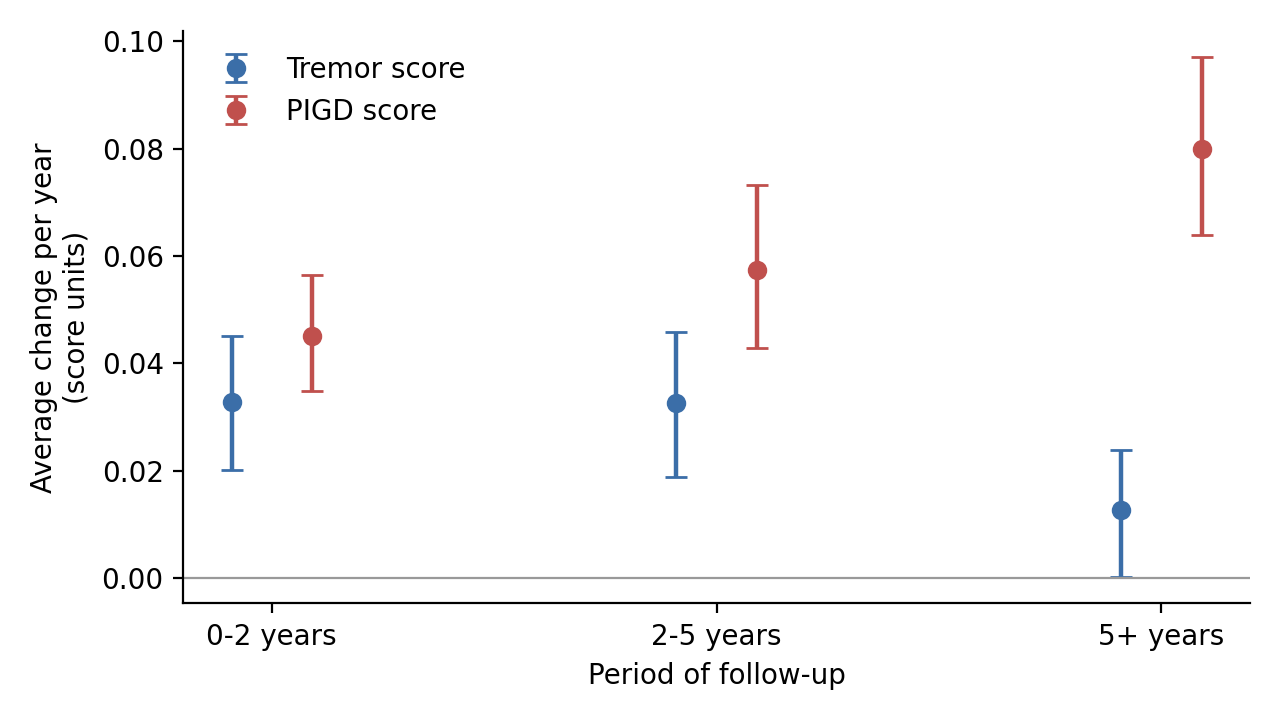
\includegraphics[width=0.84\textwidth]{s06_slopes.png}
\caption{Period-specific population slopes of the tremor and PIGD subscores under
the linear-spline mixed model. The PIGD rate accelerates and the tremor rate
decelerates over follow-up; the Wald intervals shown are too narrow by factors of
1.7 and 2.2 against a patient bootstrap.}
\label{sfig:slopes}
\end{figure}

% --------------------------------------------------------------------
\section{Discrete latent clinical states}
\label{sup:clinical}
% --------------------------------------------------------------------

Section~\ref{sec:richer} reports that a discrete latent state over ten clinical
measurements predicts the next label substantially \emph{worse} than the subtype
history alone. Table~\ref{stab:clinical} gives the full comparison.

State count was selected on a 280-patient development set by held-out next-visit
log-density, which improves monotonically from two to eight states; six states
were chosen by the one-standard-error rule and eight by the maximum. The fits are
multimodal from four states upward, with the spread of the training
log-likelihood across random starts exceeding 1,000 nats.

On 2,091 identical two-class cases the six-state model reaches 0.7255 and the
eight-state model 0.7336, against 0.8384 for the subtype-history model: paired
differences of $-0.1130$ and $-0.1048$, both intervals excluding zero. The loss is
concentrated where the current label is PIGD, with accuracy 0.397 against 0.787
and PIGD recall 0.218 against 0.659.

The bottleneck, not the measurements, is responsible. A direct logistic model on
the same ten measurements and the interval reaches 0.8307 with the \emph{best}
Brier score and log loss of any model on that evaluation set --- $+0.1052$ over
the latent model, and indistinguishable from the subtype-history model
($-0.0077$, $-0.0204$ to $+0.0046$). Restricting it to the tremor and PIGD scores
alone changes nothing ($-0.0010$, $-0.0114$ to $+0.0091$), so eight of the ten
measurements add nothing to this target.

\paragraph{Interpretation.} Forcing ten continuous measurements through a handful
of discrete states orders patients by overall severity and discards the
within-patient variation the prediction needs. This experiment is the reason the
programme replaced the discrete state with the continuous per-domain profile of
Section~\ref{sec:richer}.

\begin{table}[htbp]
\centering
\caption{Discrete latent clinical states against the subtype history and against
direct models on the same measurements. $^{\dagger}$The persistence rule's log
loss is reported clipped.}
\label{stab:clinical}
\footnotesize
\setlength{\tabcolsep}{4pt}
\begin{tabular}{@{}lrlrr@{}}
\toprule
Model & Accuracy & 95\% CI & Brier & Log loss \\
\midrule
\multicolumn{5}{@{}l}{\textit{Identical 2,091 two-class cases, 627 patients with cases}}\\
Subtype-history hidden Markov model (labels only) & \textbf{0.8384} & (0.8183, 0.8568) & 0.1211 & 0.3953 \\
Persistence (last non-Indeterminate label)        & 0.8350 & (0.8147, 0.8541) & 0.1590 & $4.173^{\dagger}$ \\
Direct logistic on the ten measurements           & 0.8307 & (0.8086, 0.8515) & \textbf{0.1156} & \textbf{0.3646} \\
Direct logistic on tremor and PIGD scores only    & 0.8297 & (0.8080, 0.8495) & 0.1202 & 0.3819 \\
Latent clinical-state HMM, 6 states               & 0.7255 & (0.6960, 0.7534) & 0.1831 & 0.5493 \\
Latent clinical-state HMM, 8 states               & 0.7336 & (0.7062, 0.7607) & 0.1817 & 0.5444 \\
\midrule
\multicolumn{5}{@{}l}{\textit{Paired contrasts}}\\
\multicolumn{2}{@{}l}{Latent clinical state (6) $-$ subtype-history HMM}
   & \multicolumn{3}{l}{$-0.1130$ ($-0.1438$, $-0.0807$) \quad \textbf{excludes zero}} \\
\multicolumn{2}{@{}l}{Latent clinical state (8) $-$ subtype-history HMM}
   & \multicolumn{3}{l}{$-0.1048$ ($-0.1357$, $-0.0757$) \quad \textbf{excludes zero}} \\
\multicolumn{2}{@{}l}{Same measurements, no latent bottleneck}
   & \multicolumn{3}{l}{$+0.1052$ ($+0.0756$, $+0.1338$) \quad \textbf{excludes zero}} \\
\multicolumn{2}{@{}l}{Ten measurements $-$ subtype history}
   & \multicolumn{3}{l}{$-0.0077$ ($-0.0204$, $+0.0046$)} \\
\multicolumn{2}{@{}l}{Two label-defining scores $-$ all ten}
   & \multicolumn{3}{l}{$-0.0010$ ($-0.0114$, $+0.0091$)} \\
\midrule
\multicolumn{5}{@{}l}{\textit{Where the latent model loses: accuracy by the label recorded at the prediction point}}\\
\multicolumn{2}{@{}l}{Current TD} & \multicolumn{3}{l}{0.844 (latent) vs 0.881 (subtype history)} \\
\multicolumn{2}{@{}l}{Current Indeterminate} & \multicolumn{3}{l}{0.568 vs 0.614} \\
\multicolumn{2}{@{}l}{Current PIGD} & \multicolumn{3}{l}{\textbf{0.397} vs 0.787} \\
\bottomrule
\end{tabular}

\end{table}

\paragraph{Limitation.} The evaluation set is a 654-patient subset, so absolute
numbers differ from the 899-patient runs elsewhere in the paper; only the paired
contrasts on identical cases should be read across.

% --------------------------------------------------------------------
\section{Information criteria, boundary calls and dimensionality}
\label{sup:misc}
% --------------------------------------------------------------------

Table~\ref{stab:misc} collects three supporting analyses.

\paragraph{(a) Information criteria.} Among models sharing a joint sequence
likelihood, the hidden Markov model is preferred over a discrete chain with an
initial distribution by 224 AIC units and 186 BIC units, and over the continuous
chain by 250 AIC units. Among the chains alone the discrete chain is preferred
over the continuous one by 25 units. Among profile variants the full model is
preferred over the level-only variant by 221 AIC and 67 BIC units. \textbf{The
three groups are not mutually comparable} --- the chains' conditional pair
likelihood, the joint sequence likelihood and the profile's continuous density
are different objects --- and these criteria are in-sample and assume independent
observations, so they favour the latent layer more than clustered data warrant.

\paragraph{(b) Calls at Indeterminate visits.} At the 287 Indeterminate visits
with a defined ratio, does a model call the side of the band the ratio sits
nearer? The hidden Markov model agrees with the nearer boundary at 0.488 against
0.462 expected under independence, an excess of $+0.026$ ($-0.029$ to $+0.078$);
the profile at 0.502 against 0.471, an excess of $+0.031$ ($-0.022$ to $+0.088$).
Both intervals contain zero, as does the sensitivity analysis restricted to the
213 visits closest to a boundary. The models' \emph{probabilities} lean towards
the nearer side --- AUC 0.584 and 0.575 for ranking nearer-PIGD visits --- but
their \emph{calls} barely do. This is the same accuracy-versus-ranking
dissociation reported in the main text, seen at the one stratum that matters most.

\paragraph{(c) Dimensionality of the profile.} Seven of nine principal components
are required for 90\% of the across-patient variance of either the level or the
rate coordinates, with the first carrying 42\% and 37\% respectively and
participation-ratio effective ranks of 4.3 and 5.1
(Figure~\ref{sfig:dim}). The representation is therefore genuinely
multidimensional and not a severity score in disguise.

\begin{table}[htbp]
\centering
\caption{Information criteria, model calls at Indeterminate visits, and the
dimensionality of the nine-domain representation.}
\label{stab:misc}
\small
\setlength{\tabcolsep}{5pt}
\begin{tabular}{@{}llrr@{}}
\toprule
\multicolumn{4}{@{}l}{\textit{(a) Information criteria; groups are comparable only within themselves}}\\
Group & Model & $\Delta$AIC & $\Delta$BIC \\
\midrule
Joint sequence likelihood & Hidden Markov model (3 latent states) & 0.0 & 0.0 \\
                          & Discrete chain $+$ initial state      & 224.1 & 185.9 \\
                          & Continuous chain $+$ initial state    & 249.6 & 211.4 \\
\addlinespace[2pt]
Conditional pair likelihood & Markov chain, discrete-time         & 0.0 & 0.0 \\
                            & Markov chain, continuous-time       & 25.5 & 25.5 \\
\addlinespace[2pt]
Rich-profile variants     & Level $+$ rate $+$ medication         & 0.0 & 0.0 \\
                          & Level only (random walk)              & 220.8 & 66.8 \\
                          & Level $+$ rate, no medication         & 344.0 & 266.9 \\
\midrule
\multicolumn{4}{@{}l}{\textit{(b) Calls at the 287 Indeterminate visits with a defined ratio (220 patients)}}\\
Quantity & Model & \multicolumn{2}{l}{Estimate (95\% CI)} \\
\midrule
Agreement with nearer boundary & Hidden Markov model & \multicolumn{2}{l}{0.488 (0.434, 0.540)} \\
                               & Rich clinical profile & \multicolumn{2}{l}{0.502 (0.448, 0.559)} \\
Expected under independence    & Hidden Markov model & \multicolumn{2}{l}{0.462} \\
                               & Rich clinical profile & \multicolumn{2}{l}{0.471} \\
Excess over independence       & Hidden Markov model & \multicolumn{2}{l}{$+0.026$ ($-0.029$, $+0.078$)} \\
                               & Rich clinical profile & \multicolumn{2}{l}{$+0.031$ ($-0.022$, $+0.088$)} \\
\quad sensitivity set ($n{=}213$) & Hidden Markov model & \multicolumn{2}{l}{$+0.038$ ($-0.029$, $+0.103$)} \\
                               & Rich clinical profile & \multicolumn{2}{l}{$+0.062$ ($-0.002$, $+0.127$)} \\
AUC for ranking nearer-PIGD    & Hidden Markov model & \multicolumn{2}{l}{0.584 (0.516, 0.653)} \\
                               & Rich clinical profile & \multicolumn{2}{l}{0.575 (0.505, 0.640)} \\
\midrule
\multicolumn{4}{@{}l}{\textit{(c) Dimensionality of the nine-domain representation (934 patients)}}\\
Quantity & & Level & Rate \\
\midrule
First principal component, variance share & & 42.2\% & 37.2\% \\
First three components, cumulative        & & 66.3\% & 60.2\% \\
Components needed for 90\%                & & 7 of 9 & 7 of 9 \\
Participation-ratio effective rank        & & 4.34 & 5.11 \\
\bottomrule
\end{tabular}

\end{table}

\begin{figure}[htbp]
\centering
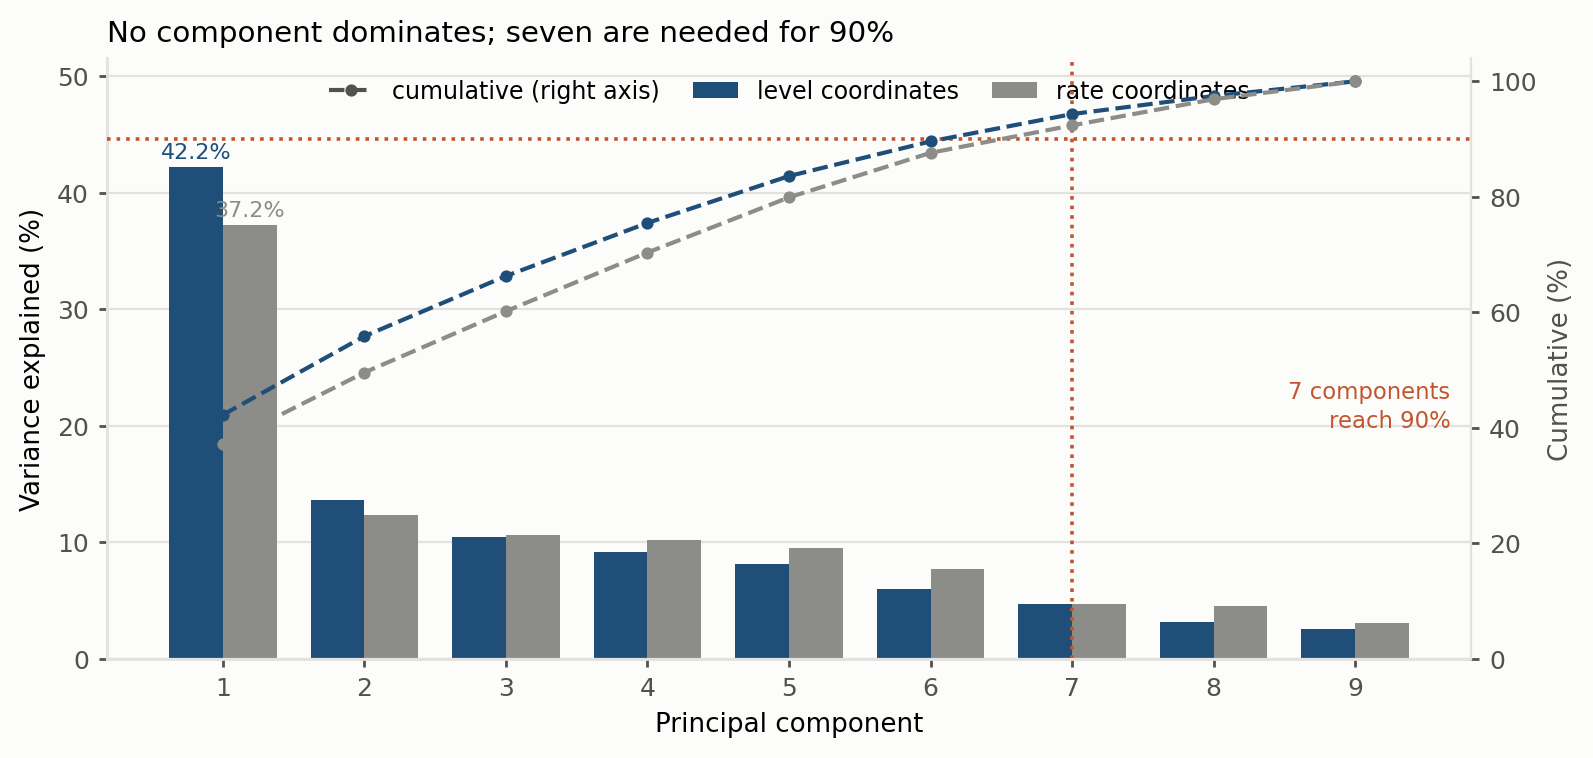
\includegraphics[width=0.74\textwidth]{s11_dimensionality.png}
\caption{Cumulative share of across-patient variance explained by successive
principal components of the profile's level and rate coordinates. Seven of nine
components are needed for 90\% of either.}
\label{sfig:dim}
\end{figure}

% --------------------------------------------------------------------
\section{Accuracy by prediction stage}
\label{sup:stage}
% --------------------------------------------------------------------

Does prediction get easier as a patient accumulates visits?
Table~\ref{stab:stage} reports two-class metrics at each prediction stage, where
stage $k$ predicts visit $k+1$ from visits $1 \dots k$, for the nine stages with
at least 66 targets.

\textbf{No change in accuracy from stage 1 excludes zero} for either model at any
reliable stage, and of 24 pre-specified paired tests exactly one interval excludes
zero: the profile's balanced accuracy at stage 1, $+0.046$ ($+0.023$ to $+0.070$),
which reflects its better PIGD sensitivity when only one visit is known and does
not persist.

Balanced accuracy does rise with stage for every model --- including the
persistence rule, from 0.717 at stage 1 to 0.816 at stage 9 --- but so does the
PIGD share of outcomes, from 23\% to 48\%. The trend is cohort composition, not
learning. Within the 225 patients observed at both early and late stages, the
late-minus-early change in accuracy is $-0.024$ ($-0.075$ to $+0.028$) for the
hidden Markov model and $-0.035$ ($-0.089$ to $+0.020$) for the profile.

\begin{table}[htbp]
\centering
\caption{Two-class metrics by prediction stage (3,017 targets of 896 patients).}
\label{stab:stage}
\small
\begin{tabular}{@{}rrrrrrr@{}}
\toprule
Stage & $n$ targets & \% PIGD & HMM acc. & Profile acc. & Persist.\ acc. & HMM bal.\ acc. \\
\midrule
1 & 835 & 23.5 & 0.8347 & 0.8455 & 0.8323 & 0.7293 \\
2 & 693 & 26.0 & 0.8644 & 0.8644 & 0.8600 & 0.8110 \\
3 & 450 & 29.3 & 0.8267 & 0.8200 & 0.8289 & 0.7799 \\
4 & 305 & 31.8 & 0.8098 & 0.8230 & 0.8033 & 0.7698 \\
5 & 200 & 34.0 & 0.8200 & 0.8350 & 0.8250 & 0.7888 \\
6 & 171 & 40.9 & 0.8304 & 0.8129 & 0.8187 & 0.8148 \\
7 & 125 & 40.0 & 0.8400 & 0.8240 & 0.8240 & 0.8200 \\
8 & 93  & 46.2 & 0.8495 & 0.8387 & 0.8602 & 0.8453 \\
9 & 66  & 48.5 & 0.8485 & 0.8485 & 0.8182 & 0.8474 \\
\midrule
\multicolumn{7}{@{}l}{Of 24 pre-specified paired tests, one interval excludes zero: the profile's balanced accuracy}\\
\multicolumn{7}{@{}l}{at stage 1, $+0.046$ ($+0.023$, $+0.070$). No change in accuracy from stage 1 excludes zero for}\\
\multicolumn{7}{@{}l}{either model at any reliable stage. Within-patient late $-$ early change in accuracy: hidden Markov}\\
\multicolumn{7}{@{}l}{model $-0.024$ ($-0.075$, $+0.028$); profile $-0.035$ ($-0.089$, $+0.020$); $n = 225$ patients.}\\
\bottomrule
\end{tabular}

\end{table}

\begin{figure}[htbp]
\centering
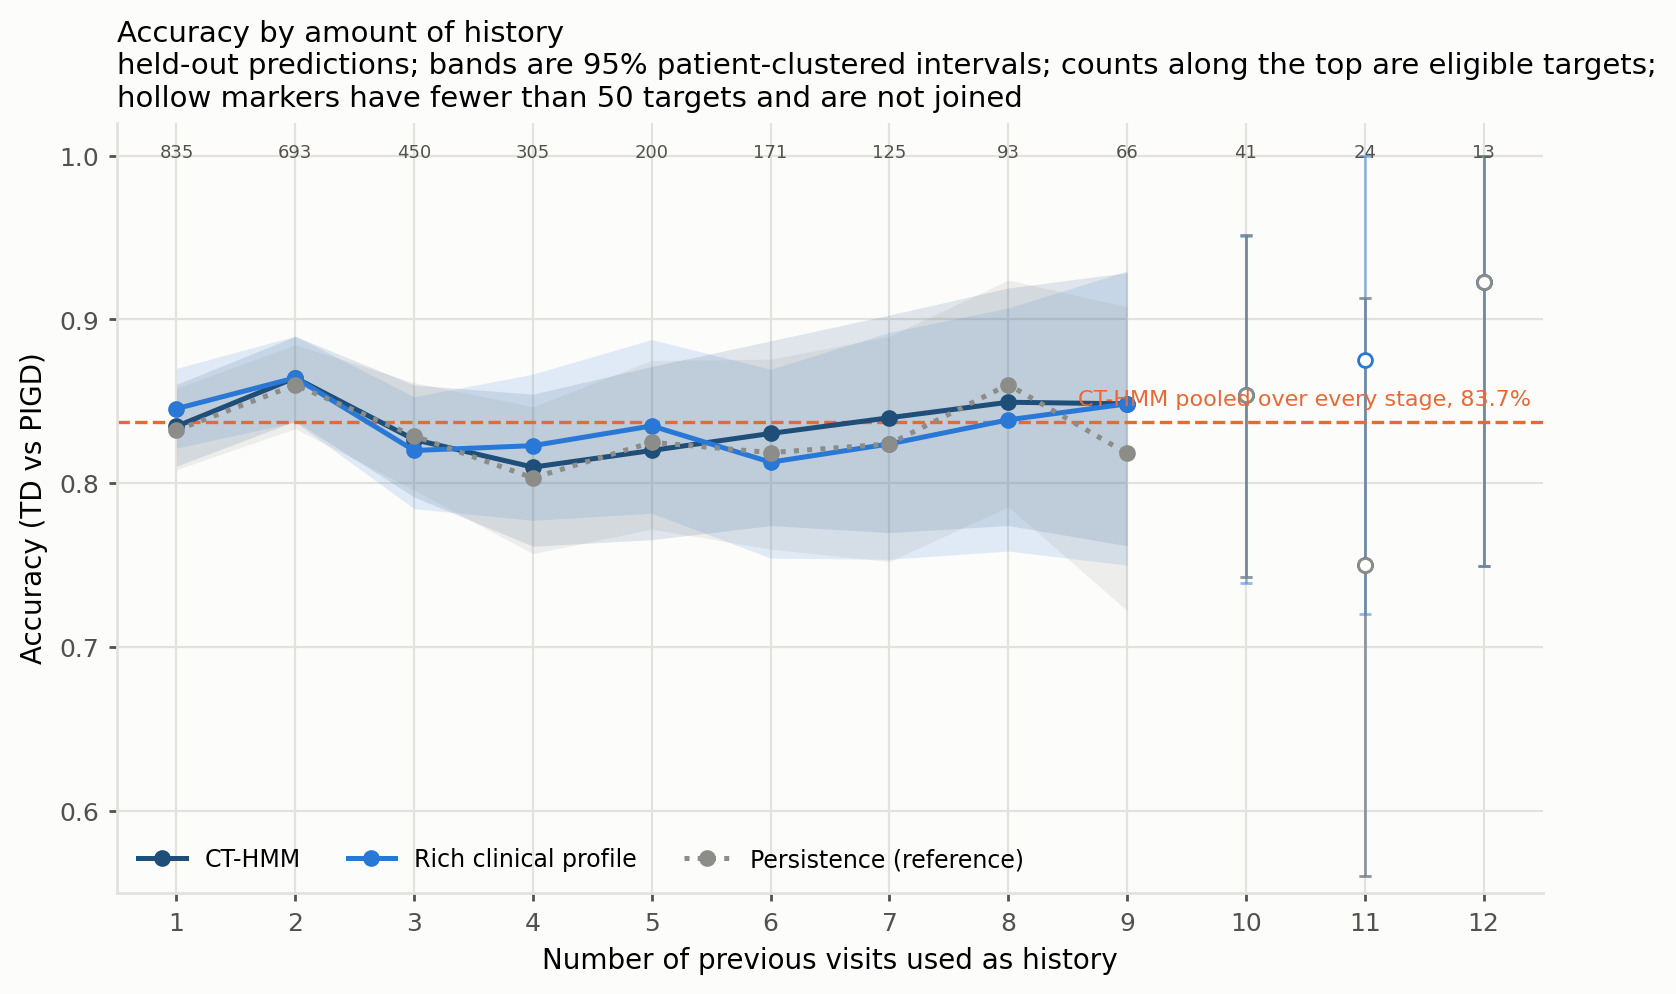
\includegraphics[width=0.80\textwidth]{s07_stage.png}
\caption{Two-class accuracy by prediction stage for the hidden Markov model, the
nine-domain profile and the persistence rule, with patient-clustered bootstrap
intervals. Late stages are small and selected on follow-up.}
\label{sfig:stage}
\end{figure}

\paragraph{Limitation.} Late stages are small and comprise patients selected on
long follow-up.

% --------------------------------------------------------------------
\section{History windows and training regime}
\label{sup:history}
% --------------------------------------------------------------------

Table~\ref{stab:history} collects the four designs that test whether the ceiling
is explained by the amount of history available or by how the model was trained.

\paragraph{Two visits are enough.} Truncating the hidden Markov model's
prediction-time history to the last two visits changes accuracy by $-0.0041$
($-0.0189$ to $+0.0100$) and AUC by $-0.0045$, both intervals containing zero;
three and five visits are likewise indistinguishable from the full record. Only a
single visit is measurably worse, by $-0.0218$ in accuracy and $-0.0617$ in AUC,
because with one visit the model has no run length to read
(Figure~\ref{sfig:windows}). The profile behaves identically.

\paragraph{Retraining on short windows is harmful.} Refitting the model on
two-visit sliding windows costs $-0.0312$ ($-0.0441$ to $-0.0183$) in balanced
accuracy, $-0.0210$ in AUC and $+0.0397$ in log loss against the full-sequence
model. A $2\times2$ design attributes the loss to the change in \emph{training}
($-0.0248$ balanced accuracy with prediction history held fixed) rather than to
the history restriction ($-0.0064$, interval containing zero). The window-trained
model falls \emph{below} persistence in balanced accuracy, through a loss of PIGD
sensitivity (0.608 against 0.706). The fitted parameters show why: the initial
Indeterminate probability falls from 0.155 to 0.044 and the Indeterminate
emission diagonal rises off its floor from 0.500 to 0.665, because a window's
first visit is treated as a draw from the initial distribution and the model
learns to explain every window's start rather than the cohort's baseline
(Figure~\ref{sfig:retrained}). Disjoint windows recover some of the AUC but halve
the training set.

\paragraph{The medication input is not doing hidden work.} Substituting the
current visit's levodopa-equivalent dose for the next visit's changes the
profile's accuracy by $-0.0013$ ($-0.0056$ to $+0.0026$), so knowing the target
visit's prescribed dose is worth nothing.

\begin{table}[htbp]
\centering
\caption{History windows and training regime, for the hidden Markov model and for
the nine-domain profile. All comparisons are paired on common targets.}
\label{stab:history}
\footnotesize
\begin{tabular}{@{}llrll@{}}
\toprule
Model & Comparison & $\Delta$ accuracy & 95\% CI & $\Delta$ AUC (95\% CI) \\
\midrule
\multicolumn{5}{@{}l}{\textit{(a) Truncated prediction history, hidden Markov model (734 common targets, 228 patients)}}\\
HMM & last 2 $-$ full (primary) & $-0.0041$ & ($-0.0189$, $+0.0100$) & $-0.0045$ ($-0.0150$, $+0.0043$) \\
HMM & last 3 $-$ full           & $+0.0027$ & ($-0.0065$, $+0.0117$) & $+0.0014$ ($-0.0032$, $+0.0061$) \\
HMM & last 5 $-$ full           & $+0.0014$ & ($+0.0000$, $+0.0043$) & $+0.0001$ ($-0.0009$, $+0.0011$) \\
HMM & last 1 $-$ full           & $-0.0218$ & ($-0.0423$, $-0.0014$) & $-0.0617$ ($-0.0858$, $-0.0385$) \\
\addlinespace[3pt]
\multicolumn{5}{@{}l}{\textit{(b) Truncated prediction history, rich clinical profile (1,489 common targets, 481 patients)}}\\
Profile & last 2 $-$ full (primary) & $-0.0007$ & ($-0.0102$, $+0.0085$) & $-0.0025$ ($-0.0069$, $+0.0016$) \\
Profile & last 3 $-$ full           & $+0.0020$ & ($-0.0062$, $+0.0096$) & $+0.0000$ ($-0.0030$, $+0.0030$) \\
Profile & current-visit medication substituted & $-0.0013$ & ($-0.0056$, $+0.0026$) & $+0.0003$ ($-0.0008$, $+0.0014$) \\
\addlinespace[3pt]
\multicolumn{5}{@{}l}{\textit{(c) Retraining the hidden Markov model on two-visit windows (2,192 common targets, 742 patients)}}\\
\multicolumn{2}{@{}l}{Window-trained, last 2 $-$ full-trained, full (primary)} & $-0.0082$ & ($-0.0193$, $+0.0026$) & $-0.0210$ ($-0.0301$, $-0.0120$) \\
\multicolumn{2}{@{}l}{\quad training effect, history fixed} & $-0.0064$ & ($-0.0155$, $+0.0027$) & $-0.0127$ ($-0.0197$, $-0.0060$) \\
\multicolumn{2}{@{}l}{\quad history effect, training fixed} & $-0.0018$ & ($-0.0089$, $+0.0054$) & $-0.0084$ ($-0.0144$, $-0.0026$) \\
\multicolumn{5}{@{}l}{Balanced accuracy, primary contrast: $-0.0312$ ($-0.0441$, $-0.0183$); PIGD sensitivity 0.608 vs 0.706.}\\
\addlinespace[3pt]
\multicolumn{5}{@{}l}{\textit{(d) The same two designs for the rich clinical profile}}\\
Profile & last 1 $-$ full history   & $-0.0139$ & ($-0.0221$, $-0.0057$) & $-0.0105$ ($-0.0150$, $-0.0062$) \\
Profile & last 2 $-$ full history   & $+0.0046$ & ($-0.0031$, $+0.0123$) & $-0.0026$ ($-0.0060$, $+0.0008$) \\
\multicolumn{2}{@{}l}{Window-trained $-$ full-trained (profile)} & $-0.0040$ & ($-0.0157$, $+0.0083$) & --- \\
\bottomrule
\end{tabular}

\end{table}

\begin{figure}[htbp]
\centering
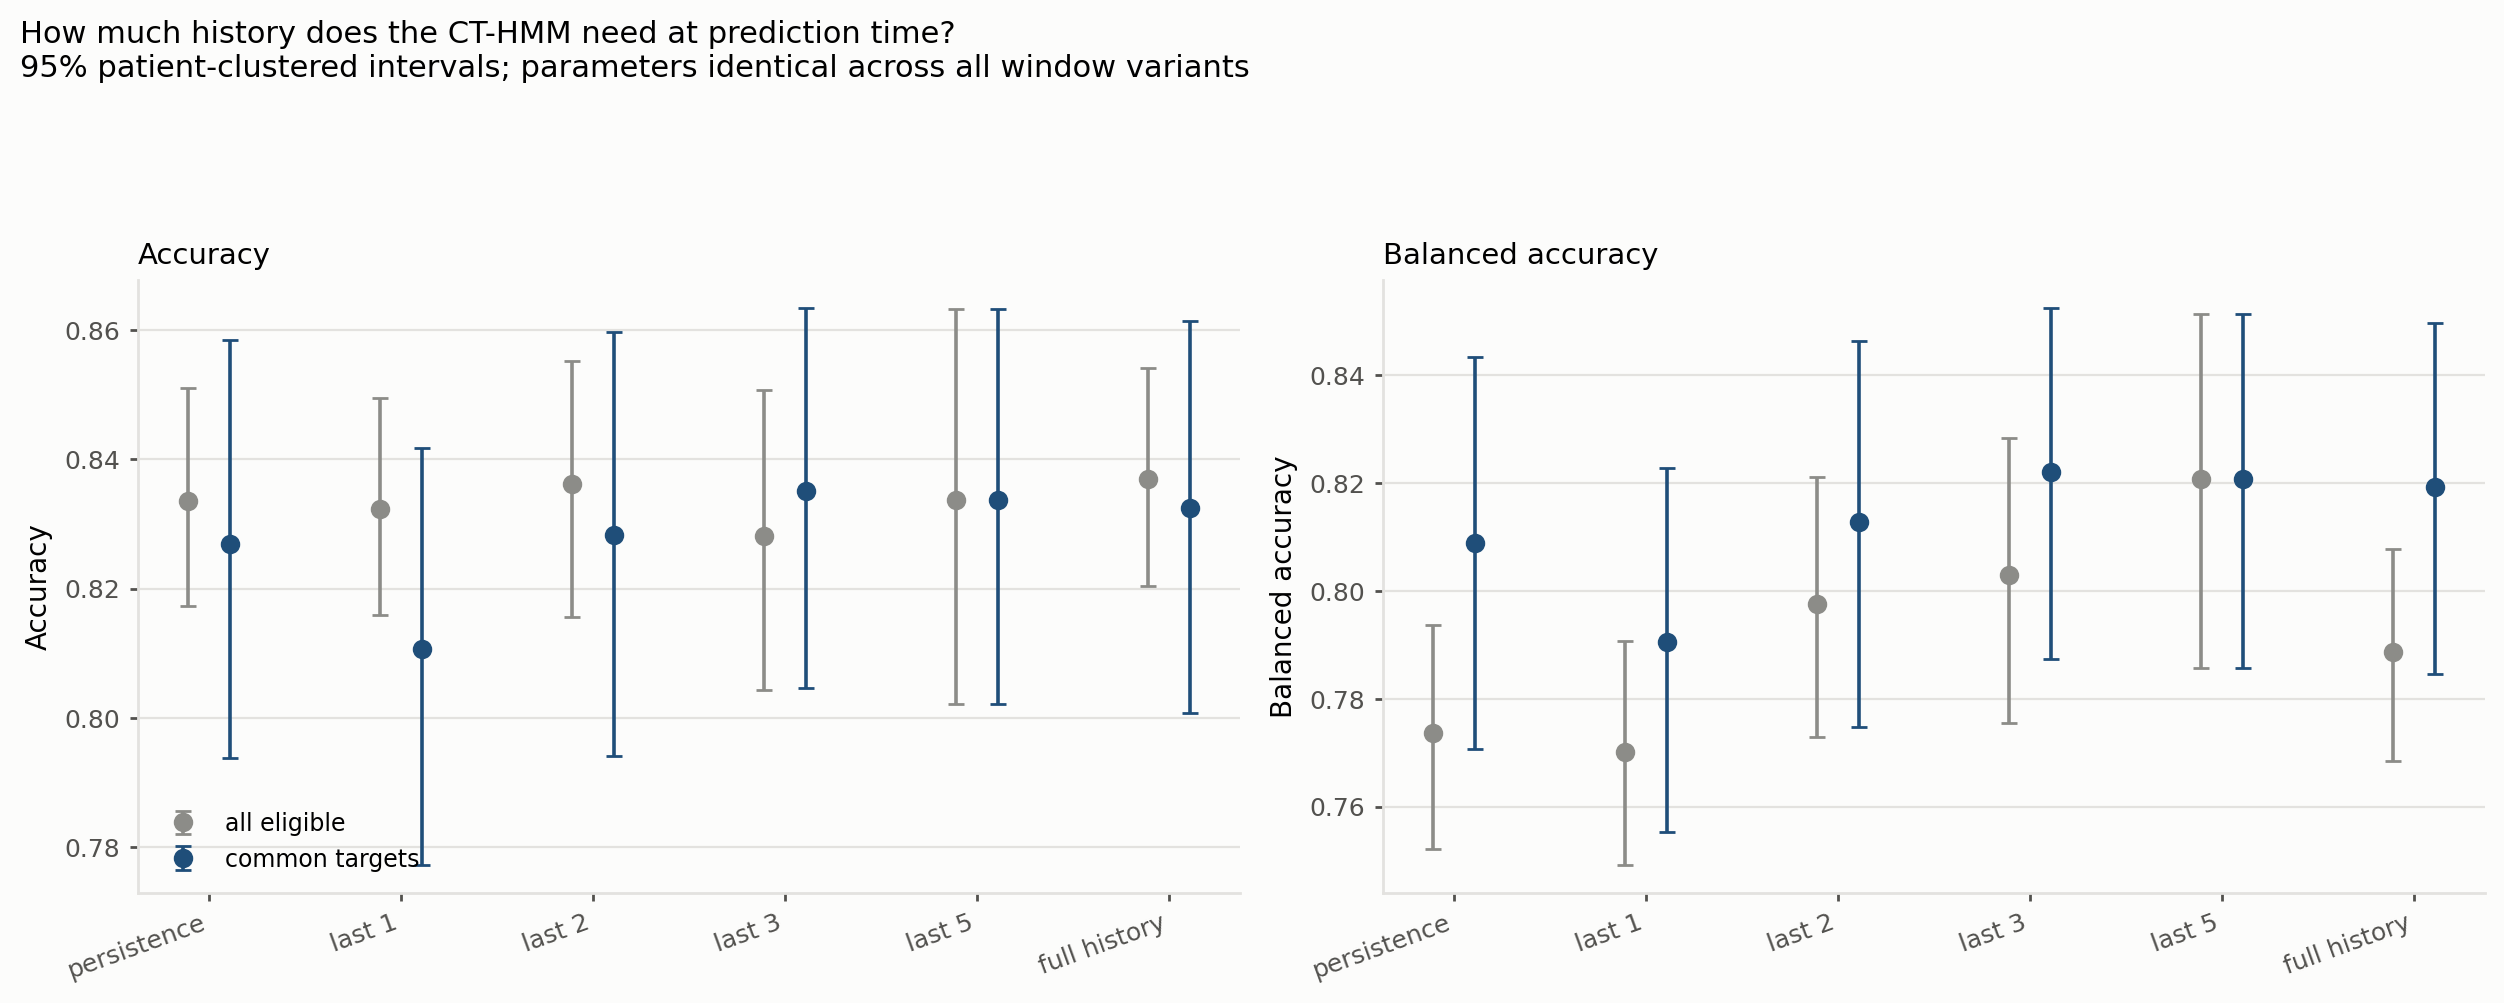
\includegraphics[width=0.80\textwidth]{s08_windows.png}
\caption{Hidden Markov model accuracy by prediction history window, on all
eligible targets and on the common targets every window can score. Only the
single-visit window is measurably worse than the full history.}
\label{sfig:windows}
\end{figure}

\begin{figure}[htbp]
\centering
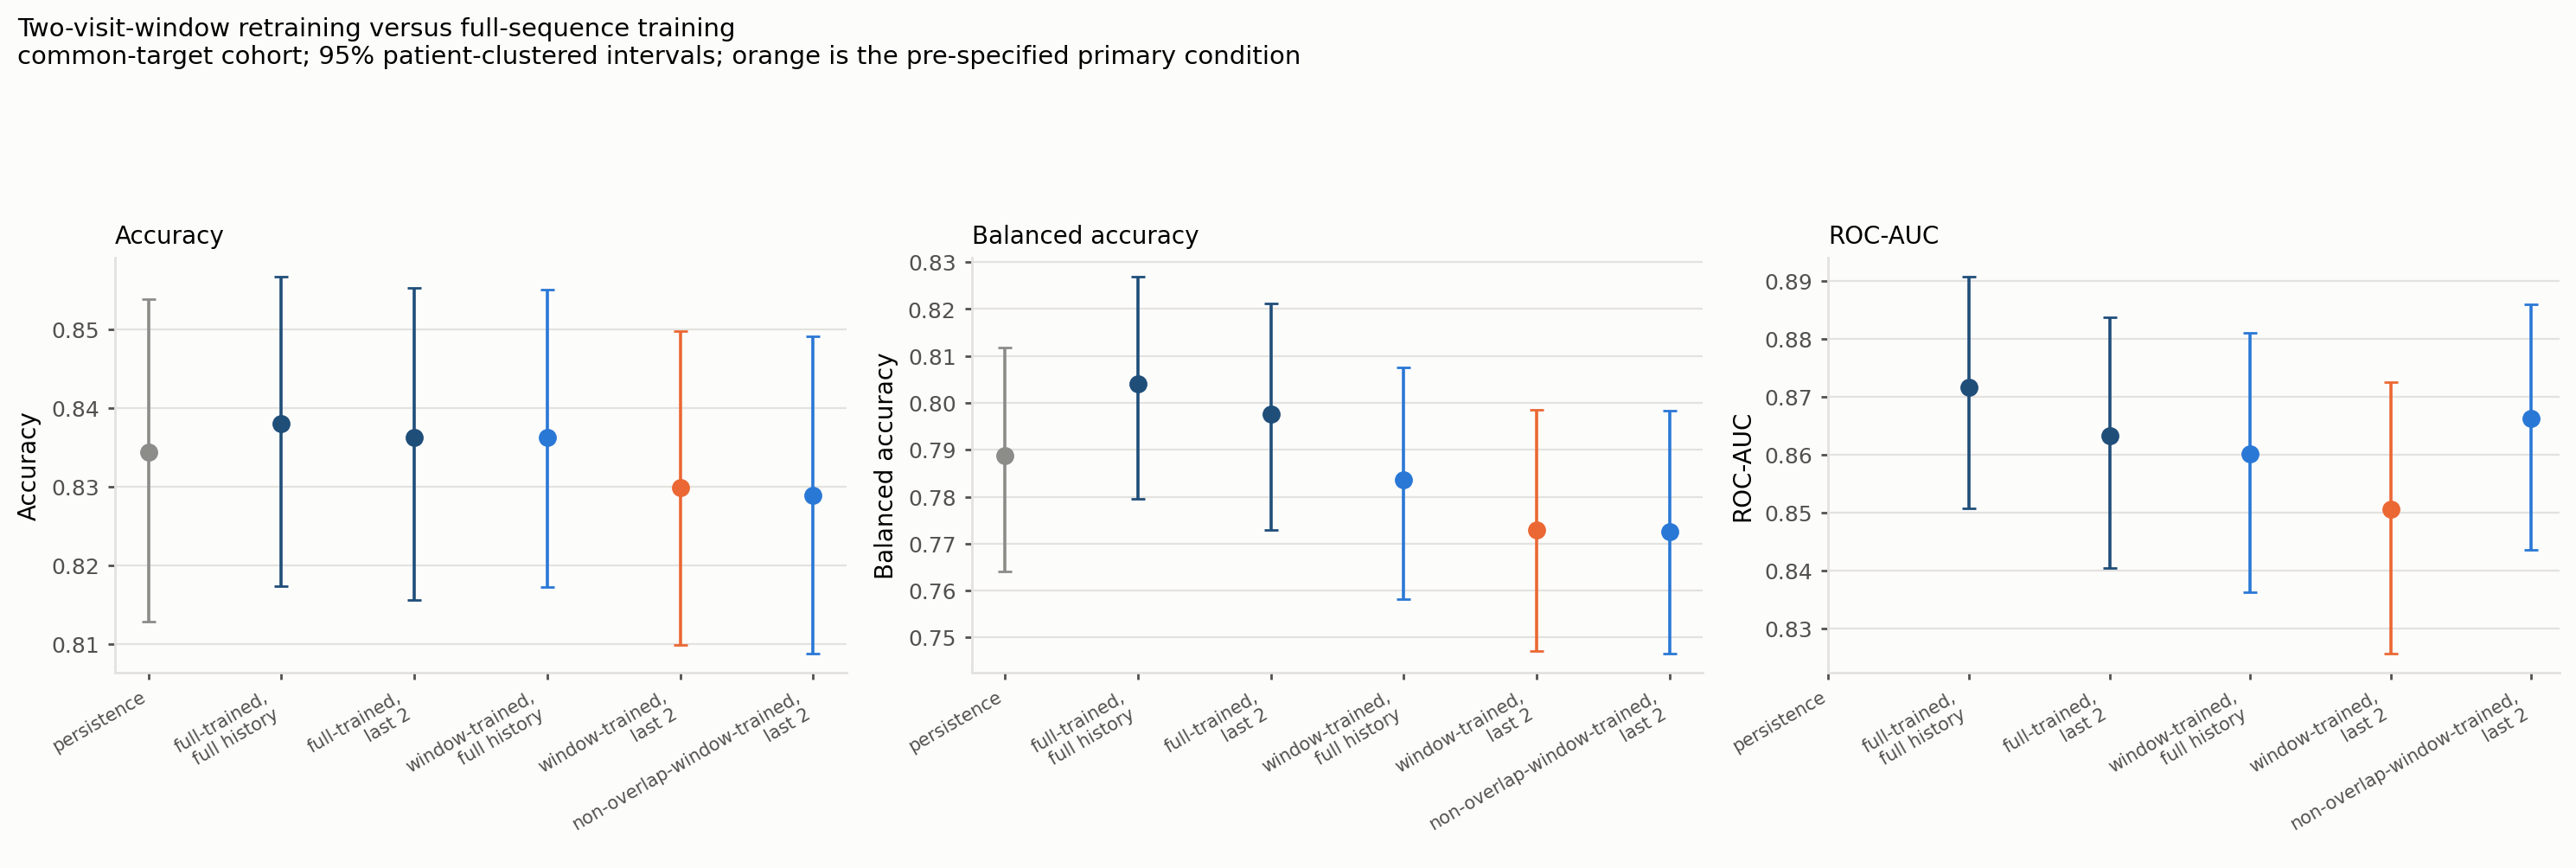
\includegraphics[width=0.84\textwidth]{s09_retrained.png}
\caption{The two-by-two design crossing training regime (full sequences or
two-visit windows) with prediction history (full or last two). The loss is
attributable to the training regime, not to the history restriction.}
\label{sfig:retrained}
\end{figure}

\paragraph{Limitation.} The common cohort for the history-window comparison is the
228 patients with at least six visits, a group selected on long follow-up.

% --------------------------------------------------------------------
\section{Patient-level accuracy}
\label{sup:patient}
% --------------------------------------------------------------------

Visit-level accuracy over-weights patients with long follow-up.
Table~\ref{stab:patient} recomputes every condition at the patient level.

Mean per-patient accuracy is 0.834 (0.817--0.852) against a visit-level 0.839,
but the distribution is bimodal: 63.7\% of patients are predicted correctly at
every eligible visit and 5.0\% at none, with a median of 1.000.

The mode a patient falls in is set by the composition of their recorded target
labels. Patients whose targets are all TD are predicted at 0.944 (persistence
0.970), all PIGD at 0.811 (0.733), majority TD at 0.684 (0.670), majority PIGD at
0.592 (0.541), and evenly split at 0.468 (0.480). \textbf{The persistence rule
shows the same gradient}, so this describes the label sequence rather than model
behaviour.

Per-patient PIGD sensitivity averages 0.550, rising to 0.722 among the 225
patients with at least two PIGD targets, where the share of patients with no
correct PIGD prediction falls from 32.5\% to 6.2\%. TD specificity averages 0.858.

At the patient level the paired comparisons repeat the visit-level ones, with 660
to 828 of the matched patients unchanged under every contrast; the models move at
most a few per cent of patients in either direction relative to persistence.

\begin{table}[htbp]
\centering
\caption{Patient-level accuracy: distribution, composition groups, class-specific
rates and paired comparisons.}
\label{stab:patient}
\small
\begin{tabular}{@{}lrrrrr@{}}
\toprule
\multicolumn{6}{@{}l}{\textit{(a) Distribution of per-patient two-class accuracy}}\\
Condition & $n$ patients & Visit-level & Mean patient & Median & \% perfect \\
\midrule
Profile, full history   & 898 & 0.8391 & 0.8342 & 1.000 & 63.7 \\
Profile, last 2 visits  & 740 & 0.8425 & 0.8395 & 1.000 & 68.2 \\
Profile, last 1 visit   & 898 & 0.8252 & 0.8219 & 1.000 & 63.3 \\
Persistence             & 898 & 0.8338 & 0.8307 & 1.000 & 63.1 \\
\multicolumn{6}{@{}l}{Profile, full history: 5.0\% of patients correct at no visit; 8.2\% below 50\%; 70.9\% at 80\% or better.}\\
\midrule
\multicolumn{6}{@{}l}{\textit{(b) Per-patient accuracy by the composition of that patient's recorded target labels}}\\
Composition & $n$ patients & $n$ targets & Profile & Persistence & \\
\midrule
All TD targets      & 510 & 1,461 & 0.9444 & 0.9697 & \\
Majority TD         & 105 & 600   & 0.6838 & 0.6704 & \\
Evenly split        & 60  & 188   & \textbf{0.4685} & \textbf{0.4799} & \\
Majority PIGD       & 61  & 333   & 0.5921 & 0.5413 & \\
All PIGD targets    & 162 & 439   & 0.8112 & 0.7330 & \\
\midrule
\multicolumn{6}{@{}l}{\textit{(c) Per-patient class-specific rates}}\\
\multicolumn{2}{@{}l}{Mean PIGD sensitivity, all patients with PIGD targets} & \multicolumn{2}{r}{0.5503} & \multicolumn{2}{l}{(persistence 0.4679)} \\
\multicolumn{2}{@{}l}{\quad among patients with $\geq 2$ PIGD targets} & \multicolumn{2}{r}{0.7222} & \multicolumn{2}{l}{(persistence 0.6537)} \\
\multicolumn{2}{@{}l}{Mean TD specificity} & \multicolumn{2}{r}{0.8583} & \multicolumn{2}{l}{(persistence 0.8834)} \\
\midrule
\multicolumn{6}{@{}l}{\textit{(d) Patient-level paired comparisons (mean difference, patients improved / worsened / unchanged)}}\\
\multicolumn{2}{@{}l}{Last 1 vs full history} & $-0.0123$ & \multicolumn{3}{l}{($-0.0225$, $-0.0017$); 46 / 78 / 774} \\
\multicolumn{2}{@{}l}{Last 2 vs full history} & $+0.0080$ & \multicolumn{3}{l}{($-0.0000$, $+0.0164$); 41 / 30 / 669} \\
\multicolumn{2}{@{}l}{Window-trained vs full-trained} & $-0.0040$ & \multicolumn{3}{l}{($-0.0157$, $+0.0083$); 36 / 44 / 660} \\
\multicolumn{2}{@{}l}{Full history vs persistence} & $+0.0029$ & \multicolumn{3}{l}{($-0.0078$, $+0.0141$); 72 / 58 / 768} \\
\bottomrule
\end{tabular}

\end{table}

\paragraph{Limitation.} The composition groups are defined from the outcomes and
are exploratory; nothing about severity or progression can be read from them.

% --------------------------------------------------------------------
\section{The band-width sweep}
\label{sup:bands}
% --------------------------------------------------------------------

Section~\ref{sec:richer} reports that adding the ratio band to the observation
alphabet raises ranking without raising accuracy. This section asks whether the
chosen band width was a poor one. Table~\ref{tab:bands} of the main text gives
the five-width sweep; Figure~\ref{sfig:bandwidth} plots it.

Accuracy lies between 0.832 and 0.836 at every width against 0.837 unbanded, and
every accuracy contrast includes zero. AUC-ROC is 0.874 to 0.878 across widths
against 0.859 unbanded, and every width gains AUC by an interval excluding zero.
Against the reference width of 0.10, width 0.30 is better on all three ranking
metrics by intervals that exclude zero, but the margins are a few thousandths;
against the \emph{unbanded} model, no width gains average precision or partial
AUC, the two ranking metrics that weight the operating region.

The optimum is interior and arises where the alphabet is coarse enough that every
category holds at least eight training observations: at width 0.05 the alphabet
has 73 categories and 28 of them hold fewer than ten observations, against zero
at width 0.50. Brier score, log loss and the calibration gap are all best at width
0.30 and all worse than the unbanded model's.

\paragraph{Conclusion.} The reference width was not a poor choice, the optimum is
not worth having, and \textbf{no width turns the ranking gain into an accuracy or
calibration gain}. The conclusion of the main text is insensitive to the band
width.

\begin{figure}[htbp]
\centering
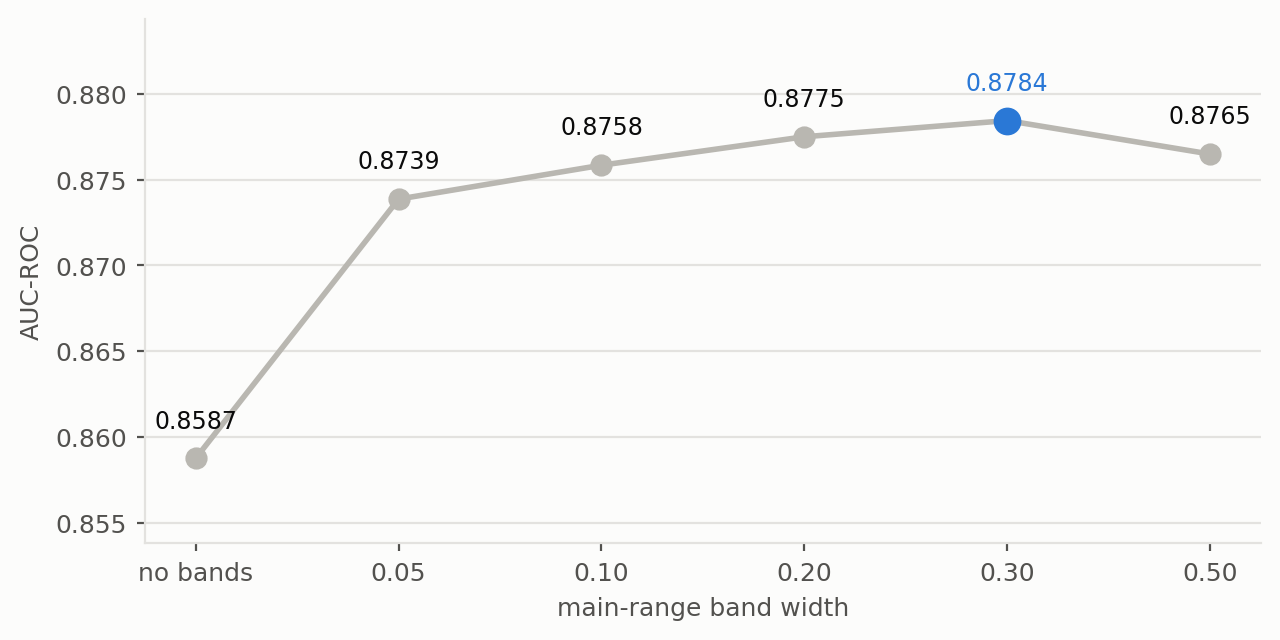
\includegraphics[width=\textwidth]{s10_bandwidth.png}
\caption{Band-width sweep: area under the ROC curve by main-range band width,
against the unbanded model at the left. Every banded width gains AUC over the
unbanded model, and the interior optimum near 0.30 (highlighted) is worth a few
thousandths of AUC over the rest. Average precision and partial AUC are in
Table~\ref{tab:bands} of the main text and do not share this optimum.}
\label{sfig:bandwidth}
\end{figure}

\paragraph{Limitations.} Five widths; the tail structure is common to all arms;
the sweep is a sensitivity analysis and was not pre-registered as a selection.

% --------------------------------------------------------------------
\section{Complete analysis inventory}
\label{sup:inventory}
% --------------------------------------------------------------------

Table~\ref{stab:inventory} lists every analysis in the programme that bears on the
question of this paper, with its cohort, its status and where it is reported. The
table is the completeness record for the study: every completed analysis appears
either in the main text or in this supplement, and the two analyses that were
specified but never run on the cohort are listed as such and described in
\ref{sup:notrun}.

Analyses belonging to a separate line of work on unsupervised structure in the
cohort are outside the scope of this paper, contribute to none of its results,
and are not listed.

\begin{small}
\begin{longtable}{@{}p{0.40\textwidth}p{0.27\textwidth}p{0.11\textwidth}p{0.14\textwidth}@{}}
\toprule
Analysis & Cohort / units & Status & Reported in \\
\midrule
\endfirsthead
\toprule
Analysis & Cohort / units & Status & Reported in \\
\midrule
\endhead
\multicolumn{4}{@{}l}{\textit{The target: how the label is built and how fragile it is}}\\
Cohort construction and participant flow & 1,080 pt / 5,774 visits & completed & \S\ref{sec:data} \\
Exact reconstruction of the label from raw items & 1,080 pt / 5,774 visits & completed & \S\ref{sec:construction} \\
Label agreement between OFF and ON examinations & 714 pt / 2,343 pairs & completed & \S\ref{sec:construction} \\
Attainable ratios on the integer lattice & 4,441 labelled visits & completed & \S\ref{sec:construction} \\
Threshold-placement sensitivity & 1,080 pt / 4,441 visits & completed & \S\ref{sec:construction} \\
\addlinespace[3pt]
\multicolumn{4}{@{}l}{\textit{The dynamics of the label, measured before any model}}\\
Transition structure, reversion, conversion, interval dependence & 934 pt / 3,361 transitions & completed & \S\ref{sec:dynamics} \\
First-order Markov property in the recorded label & 2,427 triples & completed & \S\ref{sec:dynamics} \\
Pre-registered audit of the Indeterminate class & 934 pt & completed; inconclusive by its own rule & \S\ref{sec:dynamics}, \ref{sup:ind} \\
Lag-1 autocorrelation of within-patient residual change & 397 pt / 2,050 pairs & completed & \S\ref{sec:dynamics} \\
\addlinespace[3pt]
\multicolumn{4}{@{}l}{\textit{Can a generative model of the ratio reproduce the label?}}\\
Pre-registered posterior-predictive label check & 821 pt / 3,528 visits & completed; negative & \S\ref{sec:ppc} \\
Diagnostic localisation of the misfit & 821 pt / 3,528 visits & completed; descriptive & \S\ref{sec:ppc}, \ref{sup:ppc} \\
\addlinespace[3pt]
\multicolumn{4}{@{}l}{\textit{Models of the label itself}}\\
Chains and the latent-state model on one split & 1,002 held-out pairs & completed & \ref{sup:hmm} \\
Leave-one-patient-out three-class prediction & 934 pt / 3,361 transitions & completed & \S\ref{sec:discrete} \\
Uniqueness of the fitted optimum; configuration sensitivity & 934 pt / 3,361 & completed & \ref{sup:hmm} \\
Five latent states & 934 pt / 3,361 & completed; negative, 404/934 folds converged & \S\ref{sec:discrete}, \ref{sup:hmm} \\
Prediction with no history (first-visit model) & 1,002 held-out rows & completed & \ref{sup:firstvisit} \\
\addlinespace[3pt]
\multicolumn{4}{@{}l}{\textit{Models of the continuous quantity the label is cut from}}\\
Hierarchical Bayesian growth model of the ratio & 821 pt; 825 matched pairs & completed & \S\ref{sec:continuous} \\
Student-t slope and residual variants & 821 pt / 7 splits & completed & \ref{sup:studentt} \\
Gaussian-process regression of the ratio & 821 pt / 2,707 points & completed & \S\ref{sec:continuous} \\
Independent Gaussian processes on the two subscores & 934 pt / 3,361 points & completed & \S\ref{sec:continuous} \\
Joint bivariate mixed model of the subscores & 934 pt / 8,590 obs & completed & \ref{sup:subscore} \\
Multi-output Gaussian processes & 934 pt / 3,361 points & completed & \ref{sup:subscore} \\
Fifteen-arm held-out subscore comparison & 934 pt / 3,361 points & completed & \ref{sup:subscore} \\
Time-varying spline model of the subscore rates & 934 pt & completed & \ref{sup:temporal} \\
Identifiability and interval audit of that model & 934 pt & completed & \ref{sup:temporal} \\
\addlinespace[3pt]
\multicolumn{4}{@{}l}{\textit{The harmonised comparison}}\\
Fourteen specifications under one decision rule & 934 pt / 3,361 transitions & completed & \S\ref{sec:harmonised} \\
Decomposition of each margin by current label & 934 pt / 3,361 transitions & completed & \S\ref{sec:harmonised} \\
\addlinespace[3pt]
\multicolumn{4}{@{}l}{\textit{Does a richer observation help?}}\\
Two-class next-visit prediction, seven models & 899 pt / 3,029 transitions & completed & \S\ref{sec:richer} \\
Discrete latent state over ten clinical measurements & 654 pt / 2,091 cases & completed; negative & \S\ref{sec:richer}, \ref{sup:clinical} \\
Continuous level-and-rate profile over nine domains & 934 pt / 3,353 predictions & completed & \S\ref{sec:richer} \\
Profile-derived label against the latent-state model & 898 pt / 3,020 transitions & completed & \S\ref{sec:richer} \\
Information criteria within likelihood families & full cohort & completed & \ref{sup:misc} \\
Threshold-free discrimination of next-visit PIGD & 898 pt / 3,020 transitions & completed & \S\ref{sec:richer} \\
Ratio band added to the observation alphabet & 899 pt / 3,029 transitions & completed & \S\ref{sec:richer} \\
Band-width sweep over five widths & 899 pt / 3,029 transitions & completed & \S\ref{sec:richer}, \ref{sup:bands} \\
\addlinespace[3pt]
\multicolumn{4}{@{}l}{\textit{Where and when prediction fails}}\\
Model calls at Indeterminate visits & 220 pt / 287 visits & completed & \ref{sup:misc} \\
Accuracy by prediction stage & 896 pt / 3,017 targets & completed & \ref{sup:stage} \\
Truncated prediction history, latent-state model & 228 pt / 734 common targets & completed & \S\ref{sec:ceiling}, \ref{sup:history} \\
Truncated prediction history, clinical profile & 481 pt / 1,489 common targets & completed & \ref{sup:history} \\
Retraining the latent-state model on two-visit windows & 742 pt / 2,192 targets & completed; negative & \ref{sup:history} \\
Truncated history and retraining for the profile & 898 / 740 pt & completed & \ref{sup:history} \\
Patient-level distribution of accuracy & 898 pt & completed & \S\ref{sec:ceiling}, \ref{sup:patient} \\
\addlinespace[3pt]
\multicolumn{4}{@{}l}{\textit{Specified but not run on the cohort}}\\
Integer-score measurement model of the items & --- & synthetic recovery only; not run on real data & \ref{sup:notrun} \\
Re-execution saving per-visit replicate labels & --- & specified, reviewed, not run & \ref{sup:notrun} \\
\bottomrule
\end{longtable}

\end{small}
\label{stab:inventory}

% --------------------------------------------------------------------
\section{Work specified but not run}
\label{sup:notrun}
% --------------------------------------------------------------------

Two analyses were specified in full, implemented, and tested on synthetic data,
but never run on the cohort. Neither supports any result in this paper, and
neither is reported as a finding. They are recorded here because the first is the
analysis the posterior-predictive diagnostics of Section~\ref{sec:ppc} identified
as the decisive next test.

\paragraph{An integer-score measurement model of the items.} The diagnostics in
\ref{sup:ppc} attribute the generative model's failure to the integer lattice
rather than to an additional state. The implied test is a model of the item scores
themselves --- an ordinal item-response specification with adaptive
Gauss--Hermite quadrature, carrying no intermediate state --- asking whether a
measurement-faithful generator reproduces the Indeterminate share without one.
The specification passed its synthetic parameter-recovery tests. It was never run
on the cohort, so \textbf{whether such a model reproduces the label record is
unresolved}, and this paper draws no conclusion about it.

\paragraph{A re-execution saving per-visit replicate labels.} The
posterior-predictive check did not retain the per-visit replicate labels, which is
why the diagnostics in \ref{sup:ppc} are referenced to a covariate-blind
generator rather than to the patient-conditional replicate distribution the check
itself used. A protocol-compliant re-execution that would have saved them was
specified and reviewed but not run. This limits the diagnostics to a descriptive
localisation of the misfit; it does not affect the check's verdict, which is based
on the saved omnibus statistic and its pre-registered threshold.
